%
\chapter{Discussion}
\label{ch:discussion}

The discussion chapter connects the results to the theory, with focus on the aims of this work.
% Brief summary of the aims:
The overall aim is to improve the performance of SEM EDS, which is split in two parts:
($1$) to investigate performance parameters for the SEM EDS setup and the acquisition parameters, ($2$) to investigate bulk corrections for the quantification with open-source code.
A good EDS analysis requires a well functioning setup, adequate acquisition parameters, and high quality data processing routines.
The focus of this work for part ($1$) has been to find possible test metrics, describe them thoroughly in the theory chapter, and implement the metrics in code.
The main focus has been on the metrics themselves and not the acquisition of the data.
The focus for the data treatment in part ($2$) has been to implement SEM EDS bulk corrections in open-source python code, as this is not available in the community at the time of writing.
Different approaches to the bulk corrections have been tested and are discussed in this chapter.
This chapter is built up as the results chapter, i.e. first an initial qualitative analysis of the data, then the performance parameters, and finally the bulk corrections.
% DONE add: new Julia matrix corrections stuff at https://pages.nist.gov/NeXLSpectrum.jl/methods/#Matrix-Correction











\section{Qualitative analysis}
\label{discussion:qualitative_analysis}


% overview of the data
The overview spectra of GaAs and GaSb in \cref{fig:results:overviewGaSb_withArtifacts} and the voltage series in \cref{fig:results:GaAs_voltages,fig:results:GaSb_voltages} show that the acquired data is of varying quality.
Assessing the use of performance parameters on spectra of varying quality is important, as the performance parameters should be able to distinguish different quality spectra, and thus it was necessary to acquire spectra of varying quality.
The spectrum quality is affected by the beam energy and the amount of counts, which is revealed by looking at group (A) and (B), being the voltage series of GaAs and GaSb.
The $30$ kV and $15$ kV spectra are in general of good quality with high counts, not too much noise, and clear peaks.
The spectra with high amount of counts have lower relative variations in the counts, seen as a more even plot of the blue $400$ pA PT $1$ spectrum compared to the $50$ pA PT $1$ spectrum in panel (a) of \cref{fig:results:overviewGaSb_withArtifacts}.
However, the amount of artifacts also increases with the amount of counts, exemplified by this spectrum with the highest amount of counts.
An increase amount of artifacts, e.g. the internal Si fluorescence peak, is also observed in the $30$ kV spectra, compared to the other voltages in (A) and (B). 
This increase can be due to the higher count rate in the $30$ kV spectra.
The $10$ kV and $5$ kV spectra have lower counts, as the beam current was kept constant in the voltage series.
The lower counts were expected, and as seen in the voltage series figures, the $10$ kV and $5$ kV plots are visually of poorer quality.
With visually poorer quality, such as more noise and less clear peaks, the metrics and the quantification were expected to be worse.
In general the $5$ kV and $10$ kV spectra performed worse than the $15$ kV and $30$ kV spectra, which is discussed more in \cref{discussion:performance}.
As the $15$ kV and $30$ kV spectra performed better, these voltages were chosen for group C and D, where the goal was to investigate the effect of the beam current, beam energy, and process time.
These spectra all are assumed to have enough counts to be reasonably assessed with the metrics.


% linear vs log scale, artifacts
Qualitative analysis of EDS spectra are influenced by the choice of scale, i.e. linear or log scale.
AZtec has a default setting of a linear scale, with the option of a log scale.
The log scale is used in most plots in this work, as it highlights disturbances and makes the spectrum faster to assess.
This is especially true when a specimen contains trace elements, as the low peaks from the trace elements are more visible in the log scale.
The linear scale emphasizes the high peaks, making artifacts and disturbances less visible.
The coincidence peaks from the Sb L peaks visible in panel (a) of \cref{fig:results:overviewGaSb_withArtifacts} would be invisible in a linear scale, but the presence of coincidence counts lower the Fiori P/B metrics, tabulated in \cref{tab:results:fiori}.
The lower Fiori P/B ratio implies a poorer quality, as it is fewer counts in the Sb L$\alpha$ peak than it should be, and this could lead to a higher deviation in the quantification.
For GaSb spectra taken at $30$ kV, the Fiori P/B ratio is similar at PT $1$ and PT $6$ with $50$ pA beam current, and both these spectra have little coincidence counts.
In the $30$ kV, $50$ pA and PT $1$ spectrum, where the coincidence rate is high, the Fiori P/B ratio is lower for Ga K$\alpha$, Sb L$\alpha$, and Sb L$\beta$.
In the same spectrum, the amount of coincidence counts from Ga L$\alpha$ does not increase, and this Fiori P/B ratio is similar to the other $30$ kV spectra.
The log scale reveals the coincidence peaks, which is the source of the lower Fiori P/B ratio.


Another difference in the voltage series which would be hidden by a linear scale is the relative amount of counts in the background versus the peaks.
Below $2$ keV the difference between the $30$ kV and $15$ kV spectra is small, but at increasing X-ray energy the $30$ kV spectra have higher relative peak-to-background counts than the $15$ kV spectra.
Looking at the difference between the Sb L$\alpha$ peak in the $30$ kV and $15$ kV spectra, which does not have an overvoltage issue, the background increase with a factor of around $2.5$, while the peak increase with a factor of around $4$.
The Fiori P/B ratios for the voltage series support this, as the general rule seems to be that a lower beam energy gives a lower Fiori P/B ratio.
The trend of increasing Fiori ratio with increasing $E_0$ is mentioned Williams and Carter \cite[p. 614]{williams_carter_tem_2009} for TEM EDS, and is also observed in the SEM EDS data acquired.
It is not mentioned why it increase with $E_0$, only that higher ratios are better.
However, the trend is not valid for all peaks, as seen on Ga L$\alpha$ in the GaSb spectra, where the value is $86$, $110$, $113$, and $91$ for $30$, $15$, $10$, and $5$ kV respectively, all with $50$ pA and PT $6$.


As mentioned in \cref{tab:results:artifacts}, the artifacts annotated as "Coincidence 1" in \cref{fig:results:overviewGaSb_withArtifacts} are at the same energy as possible Si escape peaks from Ga K$\alpha$.
The discussion done for the coincidence peaks is equally valid if the signal has contributions from Si escape peaks.
However, the absorption probability in Si is greatest at around 2 keV, which is right above the Si K absorption edge, and because of this the ASTM 1508 state that the Si escape peak is negligible from about 8 keV \cite[8.3.2]{astm_e1508_eds_quantification}.
Additionally, the coincidence peaks marked "Coincidence 1" are quite similar to "Coincidence 2" and "Coincidence 3", which support that the peaks are coincidence peaks and not Si escape peaks.
Using a linear scale would hide artifacts like these, and it would be harder to assess which acquisition parameters give satisfactory low amounts of artifacts.
Another artifact that would be difficult to assess on a linear scale is the background.
In general, when assessing the quality of a spectrum, the log scale is therefore preferred.

% TODO discuss (?): counts vs a.u.
% \ton{Did you want a comment on plotting "a.u." instead of "counts" in the figures?}



\subsection{Artifacts}
\label{discussion:artifacts}

% artifacts
All the artifacts discovered in \cref{tab:eds_artifacts} are described in \cref{theory:eds:artifacts}.
% Noise peak and spectrum slicing (bg fit)
The noise peak around $0$ keV is present in all spectra, and is caused by the detector.
Before the model fitting the spectra were sliced after the noise peak to avoid bad fitting.
The fitting in HyperSpy is done with a polynomial background and Gaussian peaks for the lines present in the selected elements.
If too many elements are selected, e.g. adding Si because of a small Si peak, the fitted peak of the non-present element will usually have around zero intensity.
However, getting negative intensities is mathematically possible, and can occur with the model fitting in HyperSpy, which a user should be aware of.
Having peaks present in the spectrum which are not added in the model will yield a worse background fit, as the background polynomial then will compensate for the peak.
One weakness of how the model fitting was done in this project, was that the spectra was sliced off around $0.2$ keV, which removed the noise peak, but did not remove the low energy peaks of no interest, e.g. the C K$\alpha$ peak and O K$\alpha$ peak.
The HyperSpy model fitting was given either Ga and As, or Ga and Sb as the elements to fit, and the C and O peaks were not included in the model fitting.
Fitting with C and O was experimented with, but it did not give a significantly better fit, as the C and O peaks have low intensity.
Additionally, as explained below, the GaSb spectra have some low energy Sb M-lines which are not included in HyperSpy, and thus does not have a Gaussian peak fitted to them.
The model fitting done in this work was inspected visually, and the fit was considered to be good enough.
However, the fit might have been slightly better if the background fit was not affected by the low energy peaks of no interest.
The first peak of interest in this work, regarding the quantification, is the Ga L$\alpha$ peak at $1.1$ keV.
Thus, a better choice might have been to slice the spectra at e.g. $0.6$ keV, to avoid the noise peak and the low energy peaks of no interest, and still have background to fit to before the Ga L$\alpha$ peak.
% To get even better model fitting 
% To avoid bad background fits, the spectra were sliced to remove both the noise peak and the low energy peaks of no interest, e.g. the C K$\alpha$ peak and O K$\alpha$ peak.
% DONE conc: Slice off low E, at least noise, and preferably low E peaks of no interest for best fit. Slicing at E_0 or DH will give an even better fit and prevent extrapolation of the background when plotting later. Input to the fitting is: elements, E_0, and data points.

% model fit and slicing
% tailing background and use of the Duane-Hunt limit
All the spectra were acquired over $0-20$ keV, and thus the $5$ kV, $10$ kV, and $15$ kV spectra had to be sliced at both ends.
\cref{fig:results:GaAs_voltages,fig:results:GaSb_voltages}, the voltage series, show some tailing background counts, i.e. coincidence counts above $E_0$.
When using model fitting in HyperSpy, the background is fitted with a polynomial, and polynomials does not have an end.
The fitting of the background is done from zero energy to $E_0$, which is available in the metadata of the spectrum.
The energies above $E_0$ are not included in the model fitting, but the polynomial is not cut off at $E_0$.
In other words, fitting a $15$ kV spectrum recorded on a $0-20$ keV range gives nonphysical results above $15$ keV, as the background is extrapolated without any restrictions.
This is illustrated in \cref{fig:discussion:model_slicing_fit}, where the data is plotted with black dots, the fit on the whole energy range is the red line, and the fit sliced at $0.2$ keV to $15$ keV is the green line.
The red line is nonphysical, with an exponential increase of the background above $E_0$.
Visual inspections of the model fit reveals the error easily.
Slicing the spectrum correctly prevents extrapolation like this, and will even give slightly better fits.
Using the Duane-Hunt limit, discussed in \cref{discussion:duane_hunt} as the upper limit, can be useful if the specimen is charging, as the effective beam energy then is lower than the set beam energy.
Calculating the Duane-Hunt limit is also important for the fitting in HyperSpy, as the $E_0$ in the metadata is used to specify which lines are present in the spectrum.
For example, the 5 kV spectra models does not have the Ga K lines.
If the metadata is incorrect, the model fitting will yield incorrect results.
Proper input data for the fitting, i.e. the correct $E_0$ and the correct elements, as well as the relevant spectrum data points, is important to get the best possible model fit.


% absorption edge effects. suggest future work, splice
Similar absorption edge effects as observed in \cite{project_report} are present in the acquired spectra, where strong absorption edges at lower to medium energy influence the background intensities strongly.
This is illustrated well in \cref{fig:background_absorptionEdgeSi}, where the spectrum is overlaid with the mass absorption coefficient for Si.
The background intensity is reduced by the absorption edge, i.e. the intensity of the background is higher before the peak than after the peak.
This makes the background modelling more difficult, as the background is modelled with a polynomial function.
Lower accuracy in the background modelling could lead to worse quantification, as well as incorrect metrics discussed in this work.
One possible improvement to the background modelling is to use a spline function instead of a single polynomial function.
% TODO FW: model background as a spline, and use the mu_rho as a input to refine where the absorption edge could be.


% figures/discussion/model_slicing_fit.pdf
\begin{figure}[htbp]
    \centering
    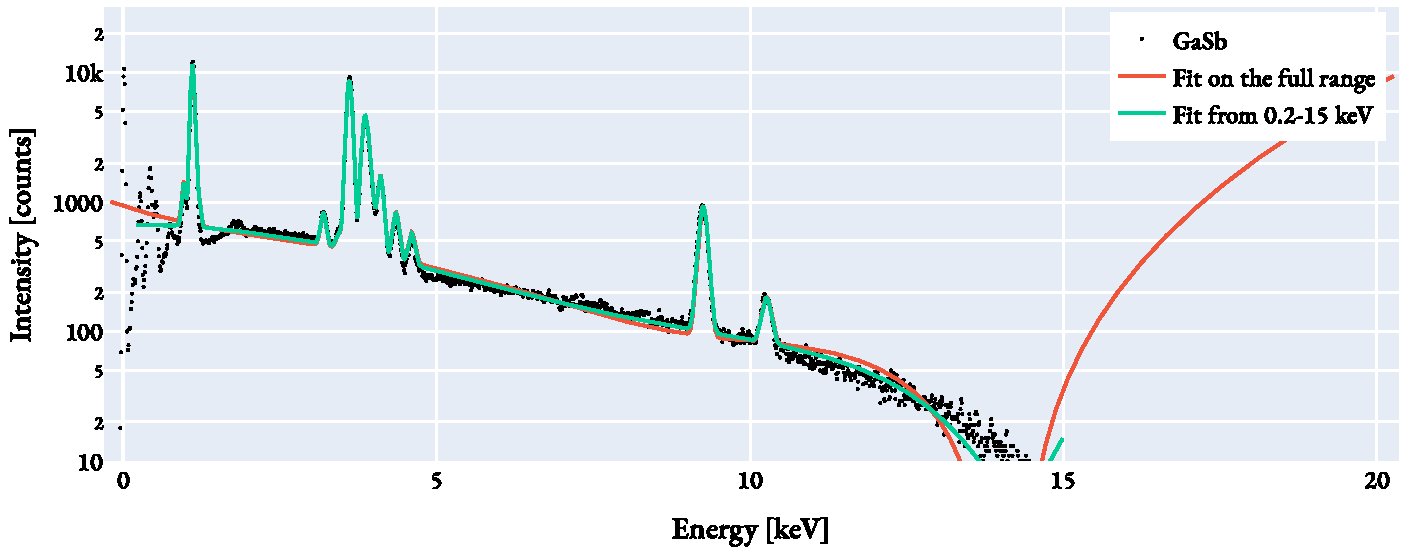
\includegraphics[width=0.85\linewidth]{figures/discussion/model_slicing_fit.pdf}
    \caption{
        Illustration of the effect of slicing the spectra before model fitting.
        Correct slicing of the spectra improve the background fit, and prevents unpredictable results above the beam energy.
        % Slicing out the noise peak and the low energy peaks of no interest will also improve the background fit.
        The sliced fit is the green line, which is not perfect at the very beginning and the end, but good enough around the peaks of interest.
        The red line is not sliced before fitting, and it fits poorly at the beginning and very poorly at the end.
        Between $5$ and $12.5$ keV the red line is also deviating more from the data than the green line.
        The red line is not too bad around the peaks of interest.
        The black dots are the data, which are from the $15$ kV $50$ pA GaSb spectrum.
    }
    \label{fig:discussion:model_slicing_fit}
\end{figure}



% More on artifacts, Si peak, C peak
% the C Ka peak. Contamination?
% no/little O Ka in GaAs.
Some artifacts seem to be affected by the amount of counts, and other artifacts are not.
As mentioned above, the coincidence events are affected by the amount of counts, giving both peaks and tailing counts.
The internal fluorescence Si peak is not affected by the amount of counts as the coincidence events are, and is present at similar low relative intensities in all spectra.
This Si peak is from the detector as explained in \cref{theory:eds:hardware}, and is expected to be present at low levels in all spectra, as SDDs have thin Si layers.
The Si signal could also have some contribution from the Si wafer that the specimens are mounted on, but this is less likely when taken into account the results in \cite{project_report}, where spectra acquired on clean Al specimen stubs had similar relative amounts of Si.
No other peaks like Fe from the column or the detector are present in the spectra.
Nor are any Ag signal present from the Ag paint used as glue to mount the specimens.
The low amount of stray signals imply that the collimator on the detector is working as intended by limiting X-rays which originate from other points than the targeted point on the specimen.
% DONE conc: low amount of stray radiation, except for C, and possible O in GaSb. The collimator is working as intended.


% C contamination
The carbon contamination in the form of a C K$\alpha$ peak is present in all spectra.
The absorption is high at low X-ray energies, but the C K$\alpha$ peak is present at similar relative intensities in all spectra.
This C peak can both be from a contamination on the specimen, or from somewhere in the chamber, detector, or column.
The most probable source is contamination on the specimen, as a post acquisition image in panel (b) of \cref{fig:SE_images:GaAs}, taken with the ET detector, showed darker spots on the acquired areas and a darker square where the specimen was scanned.
The ET detector combines SE and BSE signals, and the darker spots are therefore most likely carbon contamination on the specimen.
The image also have some horizontal lines, which are scanning artifacts.
The biggest dark spot, located highest, is from the $30$ kV spectrum, showing that the interaction volume is larger at higher beam energies.
The backscattered electrons, together with the beam electrons, are depositing C on the surface, and the backscattered electrons originates from a larger volume at higher $E_0$.
The C signal is probably from a combination of contaminations on the specimen surface, which could be plasma cleaned, and carbon present in the camber.
The source of the C signal can be further investigated by looking at different specimens, and should be done when low energy lines are of interest.
As the peaks used in this work are from $1$ keV and above, the signal from C is not of concern in the remainder of this work.
% DONE conc: C contamination from specimen or carbon in the chamber. Probably a combination, but is not an issue for the results in this work.


% O Ka peak
Another artifact observed in the spectra is the O K$\alpha$ peak, which is present in the GaSb spectra, but not in the GaAs spectra.
% However, the O K$\alpha$ peak is only present in the GaSb spectra, and not in the GaAs spectra.
The mass absorption coefficients for GaAs is twice as high at O K$\alpha$ than for GaSb, which could have been the reason for the O K$\alpha$ peak not being present in the GaAs spectra, but then the same should then have been true for the C K$\alpha$ peak.
% GaAs: mu_rho(O_Ka) = 7k, mu_rho(C_Ka) = 24k
% GaSb: mu_rho(O_Ka) = 4k, mu_rho(C_Ka) = 11k
Thus, another explanation is needed for the absence of the O K$\alpha$ peak in the GaAs spectra.
It could be due to different contamination on the two specimens, where the GaSb specimen have a thicker oxide layer than the GaAs specimen.
This can both be an effect of the As vs Sb, or the age of the specimens, as the GaSb specimen could have been exposed to air for a longer time than the GaAs specimen.
Another possibility is that the O K$\alpha$ peak is mislabeled, and is actually a Sb M-line.
This option is discussed in the next paragraph.



% Sb M-lines not in any table, but M is stated to be 0.733 keV at https://www.globalsino.com/EM/page4675.html
Another take-away from the qualitative analysis is that the HyperSpy database does not contain Sb M-lines.
The GaSb spectra have a clear peak at what is assumed to be the Sb M$\zeta$ peak around $0.42$ keV, based on the qualitative analysis AZtec, as well as the absorption edge in Sb around $0.5$ keV.
The energy of a line is located a few eV below the absorption edge.
The online book "Practical electron microscopy" by Y. Liao \cite{liao2006practical} lists a Sb M lines at $0.733$ keV, but this is only visible in the spectra as a slight increase in counts and not a real peak.
The HyperSpy database and the X-ray data Booklet \cite{thompson_x-ray_2004} does not list any M-lines below Z=$57$.
A screenshot from the AZtec software, which identifies two Sb M-lines, one at $0.4$ and a smaller at $0.7$ keV, is shown in \cref{fig:discussion:AZtec_Mlines}.
The screenshot is of the spectrum with low energy resolution, and the $0.4$ and $0.5$ keV peak is overlapping, but the AZtec software clearly identifies the leftmost part of the merged peak as a Sb M-line.
This is an indication that the peak at $0.5$ keV is not a Sb M-line, but rather that the O K$\alpha$ peak is labeled correctly.
The lack of the Sb M-lines in the HyperSpy database can be a source of error in the quantification, as the Sb M-lines are not included in the background modelling.
A solution to this is to slice off the spectrum before fitting the background so that unavailable lines are excluded from the background modelling.
This requires that the user visually inspect the lower energies thoroughly, and that the user is aware of the possibility of missing lines.
Another solution is to add the Sb M-lines to the HyperSpy database, which would require more research into M-lines of elements with Z lower than $57$.
The use of M-lines around 0.5 keV might be limited with bulk specimen, as the absorption is high, but such lines could be useful in TEM where the absorption is lower.
% DONE conc: the line is Sb M, when comparing GaAs and GaSb. Also, Sb have M lines, but not tabulated values.
% TODO FW: investigave the occurance and possible use of M-lines for Z<57. Could at least be useful for TEM, where the absrption in the specimen is lower.

\begin{figure}[htbp]
    \centering
    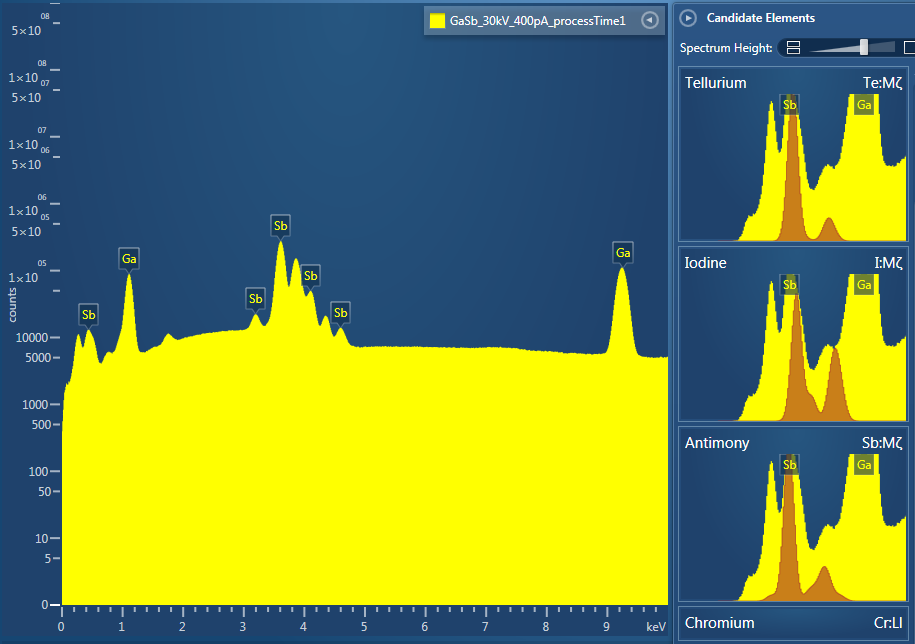
\includegraphics[width=0.99\linewidth]{figures/discussion/AZtec_Mlines.png}
    \caption{
        Screenshot from the AZtec software, showing the Sb M-lines identified at 0.4 and 0.7 keV.
        The right part of the screenshot show that tellurium and iodine match slightly better than antimony, but the L-lines present are definitely from antimony.
    }
    \label{fig:discussion:AZtec_Mlines}
\end{figure}





\subsection{Test specimen and scratched surfaces}
\label{discussion:test_specimen}

% TODO disc: test specimen, not finished.

% % test specimen
% \brynjar{not finished yet. Start with the goal of the standard, then what it may be.
% Insert suggestions for standard test specimen here.
% Not pure? Pure will give high Fiori.
% Bulk, and wafer, since it is easily available.}


BAM (Federal Institute for Materials Research and Testing) has a test sample for SEM EDS with a accompanying software, which satisfies the ISO 15632 standard.
However, the price per 28.02.2023 for this sample (EDS TM002) is $334$ EUR and $335$ EUR for the software.
A full test in accordance with the ISO standard could probably be done with a cheaper sample and a Jupyter Notebook, where the user would see all the steps and the results.
This has not been a main focus in this work, but some parameters in the ISO standard are covered in this work.
\url{https://webshop.bam.de/webshop_de/eds-tm002.html}

% paper at \url{https://www.cambridge.org/core/services/aop-cambridge-core/content/view/17A1D769BB6B9B76B5AC815911FAE7FD/S1431927613008271a.pdf/check-and-specification-of-the-performance-of-eds-systems-attached-to-the-sem-by-means-of-a-new-test-material-eds-tm002-and-an-updated-evaluation-software-package-eds-spectrometer-test-version-3-4.pdf}



% geometries - per erik. looking at surface or cross sections. rough surface
% short comment on scratched surface
The GaSb specimen, as shown in the overview image in \cref{fig:SE_images:Overview_GaAs_GaSb}, has a scratched surface.
According to the standards ISO 22309 \cite{iso_quantification_22309} and ASTM E1508 \cite{astm_e1508_eds_quantification} on SEM EDS quantification, EDS analysis of non-flat surfaces, e.g. scratched surfaces, gives a higher uncertainty in the quantification.
The ASTM standard claims that analysis of "casual" surfaces give unpredictable variations in the quantification.
SEM EDS analysis of non-flat and non-polished surfaces are of huge interest and are probably done quite frequently, thus investigating possible corrections for non-flat surfaces would be of great interest.
Newbury and Ritchie \cite{newbury_ritchie_2013_flatness} used Monte Carlo simulations to investigate how rough a surface can be before severely increasing the uncertainty of quantification, and they conclude that uneven surfaces with $100$ nm repeated variations can increase the relative error with $5$ \% or more.
The scratched areas analyzed in this work was only used as a reference to the flat areas, for a brief comparison of the AZtec results.
The deviation from $50:50$ was around $10$ at.\% for the scratched areas.
Establishing corrections for non-flat surfaces would require more data.
Such corrections would probably both be dependent on the surface and the material, as the issue with non-flat surfaces is that the X-rays are absorbed more or less depending on the path length through the material, which is dependent on the surface.
The first step towards non-flat corrections would be to get open-source bulk corrections working properly for flat surfaces, thus the focus was directed on the flat areas.
% TODO FW: non-flat corrections, which migt be very useful, but probably requires lots of work. First step is getting open-source bulk corrections working properly for flat surfaces, which should be documented well so that further work is easier to do.








\section{EDS performance parameters}
\label{discussion:performance}

% TODO disc: order for performance parameters. Both sentence below and headers.
The metrics measured to evaluate the performance of the detector and the acquisition parameters are the energy resolution, the scale, the offset, the peak deviations in calibrated positions, the peak ratios, the Duane-Hunt limit and the Fiori peak-to-background ratio.
Additionally, observations for PT, $E_0$, and $i_b$ are discussed.



\subsection{Energy resolution}
\label{discussion:energy_resolution}


% the first table with energy resolution in a spectrum
\cref{results:performance} begins with a table showing an issue with the calculated energy resolution, which is that a single spectrum gives different energy resolutions when using different reference peaks in the calculation.
The energy resolutions are calculated from the FWHM of different peaks, using \cref{eq:estimateFWHM} by Fiori and Newbury.
Calculated energy resolutions for GaAs and GaSb taken at $30$ kV with $50$ pA is tabulated in \cref{tab:results:lines_info_30kV_50pA}.
The calculated energy resolutions for GaAs varies from $123$ eV to $135$ eV, and for GaSb from $121$ eV to $133$ eV,  when using different peaks as the reference peak.
This illustrates an issue with specifying a single energy resolution for a spectrum.
The energy resolution is supposed to be a property of the detector.
As explained in the theory chapter, the acquisition parameters like ICR and PT affect the achieved energy resolution, but the results here show that the specimen and choices for calculations also affect the energy resolution.
%  data here shows that the energy resolution is also affected by the specimen.
The ISO standard 15632 \cite{iso_qc_15632} on SEM EDS performance parameters is directed towards the manufacturer of the detector, where the described method for measuring the energy resolution is with an $^{55}$Fe source off the microscope.
However, for user laboratories the standard specify that a polished manganese specimen can be used.
This does require that the user laboratory has a polished manganese specimen, which is not the case for the user laboratory in this work.
% Possible test specimen is discussed in \cref{discussion:other:test_specimen}.


Measuring directly on a Mn specimen is the first of three possibilities for measuring the energy resolution, introduced in \cref{theory:eds_performance:energyres}.
The second method is to measure the FWHM of Ni K$\alpha$, e.g. with a NiO test specimen from Ted Pella, and then multiply the FWHM by $0.926$ to get the approximate FWHM of Mn K$\alpha$.
This method relies on specific specimen, which can be expensive and had been ordered but not delivered during the time span of this work.
Other non-standard Ni test specimen could probably be used, but the 0.926 factor is based on NiO test specimen and the results from a round-robin study in 1995 with five TEM laboratories \cite{bennett_egerton_1995}.
The third method, which is given in Goldstein \cite{goldstein_scanning_2018}, is the Fiori and Newbury equation mentioned above.
As neither a Mn specimen nor a NiO specimen was available for this project, the third method was used.
The third method is also more flexible and general, as it does not rely on specific specimen.


% TODO ? discussion: input NiO energy in the equation on try to get the 0.926 factor.


% The ISO standard
% \brynjar{ISO 15632: "The
%     resolution value shall be accompanied by a statement of count rate for which the specification is valid.
%     For most detector systems the best energy resolution is attained at an ICR < 1 000 counts/s and the
%     best energy resolution shall be specified. Where detector systems offer higher count rate capability, e.g.
%     SDD EDS, the energy resolution shall also be specified at high ICR, e.g. 50 000 counts/s, 500 000 counts/s."}

% more on energy resolution
Claiming that the energy resolution is a property of the detector, the acquisition parameters, the specimen, and additionally the choices during calculations, raises the question of what the energy resolution of a detector actually is.
The energy resolution is a much used comparison metric for EDS detectors, and is thus important.
Having a single number for the energy resolution is convenient, but it is not a complete description of the energy resolution.
Traditionally, the energy resolution is seen as a property of the detector, but the ISO standard 15632 \cite{iso_qc_15632} stress the need for specifying the ICR with the energy resolution, preferably with one number at low ICR and one at high ICR.
When looking at the other acquisition parameters, the data in \cref{tab:results:energy_resolutions} shows a strong dependence on the PT, and a weaker trend with the ICR.
These numbers are calculated with HyperSpy, which use \cref{eq:estimateFWHM}, but selects the reference peak as the alphabetically first $\alpha$ peak.
Both the use of \cref{eq:estimateFWHM} and the choice of reference peak was not documented properly, so the author of this work raised an issue\footnote{Issue: \url{https://github.com/hyperspy/hyperspy/issues/3098}} on the HyperSpy GitHub page with a suggestion for improvement with a pull request. \footnote{Pull request: \url{https://github.com/hyperspy/hyperspy/pull/3099}}.
Regarding the PT, it should be selected to give the best energy resolution, as it is safe to assume that the manufacturer has done this for the specifications of the detector.
The highest PT gave an energy resolution of $127$ eV, while the lowest PT gave $158$ eV.
The ICR trend is weaker, indicating that lower ICR gives better energy resolution, but the changes are around $\pm 2$ eV.
The ICR is dependent on the beam energy and the current, but also on the specimen.
This specimen dependence for the ICR might be one of the factors which make the energy resolution dependent on the specimen.


Another specimen factor for the energy resolution is the available lines generated by the elements.
This effect is most apparent when looking at the estimated FWHMs from multiple lines in a single spectrum, as in \cref{tab:results:lines_info_30kV_50pA}.
The shared lines, i.e. Ga L$\alpha$ and Ga K$\beta$, have similar but not identical FWHMs.
Such variations of a few eV are expected with measurement noise, and is very small compared to the peak broadening from the detector, as explained in \cref{theory:eds:hardware}.
The lowest energy resolution for both spectra is from the Ga K$\beta$ line, implying that the Ga K$\beta$ line is narrower than it is "supposed" to be, compared to the other lines.
For GaAs, the explanation could have been that the peak overlap some with As K$\alpha$, but that is not the case for GaSb, and another explanation is needed.
The Ga K$\beta$ peak is much less intense than the other lines used as reference, which can give slightly worse model fit.
Another possibility is that the equation used to estimate the FWHM works better for $\alpha$ lines, but that is contradicted by the As K$\beta$, Sb K$\beta_1$, and Sb K$\beta_2$ lines.
The most probable cause is the low intensity in the Ga K$\beta$ peak.
By cherry picking a reference line, the reported energy resolution can be lowered, but it is not good practice and it is not a general solution.
A solution for the method using \cref{eq:estimateFWHM} could be to average the estimated energy resolution for a fixed set of reference lines.
This would then depend on a standardized test specimen.
Regarding the small variations between spectra with similar or equal acquisition parameters, the cause is probably measurement noise.
Such small variations when measuring the metric are expected, and would probably be solved by averaging over multiple spectra with the same acquisition parameters.


To summarize, the energy resolution of a detector should be specified with the acquisition parameters, the specimen used for the measurement, and the method used for calculating the energy resolution.
Alternatively, a larger uncertainty can be used to specify a more general energy resolution.
An example of the first, based on the results in \cref{tab:results:energy_resolutions}, would be:  the energy resolution of the detector is $127$ eV at $30$ kV and $50$ pA, measured on a GaAs specimen, and calculated with \cref{eq:estimateFWHM} with the Ga K$\beta$ line as reference.
The second way of specifying the energy resolution would be: the energy resolution of the detector is $127 \pm 6$ eV at satisfactory acquisition parameters, measured on a GaAs and GaSb specimen, calculated with \cref{eq:estimateFWHM}.



\subsection{Scale, offset, and peak position deviations}
\label{discussion:scale_offset}

The calibration of the spectra was done with HyperSpy, and the results for the energy scale, the offset and the deviations in the peak positions are close to the expected values.
The scale and offset is presented in \cref{tab:results:scale_offset}, and the $\Delta E$ in \cref{tab:results:lines_info_30kV_50pA} are representative numbers for the peak deviations.
Low deviations for the scale and offset show that the detector is calibrated properly.
The calibration accuracy is further reinforced by the low peak deviations.
The GaAs spectra have one order of magnitude higher standard deviation for the scale than the GaSb spectra, which is probably due more $15$ kV and $30$ kV spectra for GaSb.
The numbers would probably be more similar if the same number of spectra were used for both specimens.
However, the numbers are still comparable, as the scale and offset is not expected to change with the specimen nor the acquisition parameters.
With a scale of $10$ eV, a peak position deviation of $\pm 2$ eV is good, and any better is not necessary as the channel size and energy resolution limits perfect peak position.

%
According to the responsible engineer\footnote{Verner Håkonsen, communication by mail and in person.} for the SEM Apreo at NTNU NanoLab, the calibration routine for the instrument used in this thesis is just to measure specific known reference peaks, and then the software does the calibration.
For peaks at energy from $1$ keV, this appears to be sufficient and gives good results.
However, it can be observed in panel (a) of \cref{fig:results:overviewGaSb_withArtifacts}, that low energy peaks have visual peak deviations.
The center of the C K$\alpha$ and O K$\alpha$ peaks are offset from the theoretical values, marked by vertical dashed lines.
The poorer calibration at low energies can both be due to lower amount of counts here combined with high absorption, and the calibration routine.
The calibration routine is probably not optimized for low energy peaks, as the routine is probably optimized for the most common use cases.
If a user needs higher accuracy in the lower energy region, the spectrum should be calibrated with reference peaks in the lower energy region before the analysis.
In this work, where the focus is peaks at $1$ keV and above, the calibration is sufficiently accurate.
% DONE conc: when working with peaks above 1 keV, the detector used has a well calibrated energy axis, with a scale of 10 eV and an offset of 0 eV. The peak position deviations are low. The detector is just calibrated with pure Cu and the short calibration.
% TODO FW: additional calibration routine when low energy peaks are of interest.



\subsection{Peak ratios}
\label{discussion:peak_ratios}

The idea of measuring peak ratios was to get a number for the possible carbon contamination, as it is done in the work of Egerton \cite{egerton_nio_characterization_1994}.
There is some carbon present in both the GaAs and GaSb spectra, thus the peak ratios could give a number for the carbon contamination, and the change over time.
However, a metric like this needs a time series of spectra, where the change in K to L peak ratio is plotted, and an increase in K over time would indicate carbon contamination.
Measuring time series of spectra was not prioritized in this work, as the focus was directed elsewhere.

% See absorption with peak ratios
The peak ratios in \cref{tab:results:peak_ratios} are not an example of a time series, but the ratios are still interesting.
GaSb have around three times higher ratio for Ga K$\alpha$/L$\alpha$ than GaAs.
The higher ratio either indicates more Ga K$\alpha$ or less Ga L$\alpha$ signal registered.
The GaAs spectra have much intensity from the As L$\alpha$ peak, which can be absorbed by the Ga L$\alpha$ peak, and thus giving the Ga L$\alpha$ peak a higher relative intensity in the GaAs spectra.
As explained in \cref{theory:xray_formation:characteristic}, the absorption probability is the highest right above the absorption edge.
With As L$\alpha$ right above the enery of Ga L$\alpha$, the As L$\alpha$ X-rays are absorbed easier than the Sb L$\alpha$ X-rays, and such absorption can result in more fluorescence from Ga L$\alpha$.
This is an indication of absorption, which will be discussed more in \cref{discussion:quantitative}.
% DONE conc: peak ratios can indicate absorption, at least relative absorption when comparing specimen.



% detecting artifacts as Egerton: not possible with the easy geometry of a flat wafer
One of the more interesting results which are achievable with measuring peak ratios is to get a number for the source of artifacts.
This is explained in the work of Egerton \cite{egerton_nio_characterization_1994}, where the ratio between a targeted element and a grid element outside the targeted area is investigated.
The grid element must contain a high and low energy line, and the element in the targeted area must contain a line in between the two lines in the grid element.
In the work of Egerton, which is the routine following the TED Pella NiO test specimen, the element in the targeted area is Ni and the grid element is Mo.
The idea is that a high amount of Mo K signal indicate that there are electrons from the beam which are deflected and hit the grid directly.
Backscattered electrons can also contribute to the Mo K signal, but increased amount of deflected beam electrons would certainly influence the ratio of K and L in Mo.
If there are higher amounts of Mo L signal, the source of artifacts is more likely to be from secondary fluorescence from Ni K X-rays.
Skomedal \cite{skomedal_improving_2022} investigated the use of a NiO specimen in STEM EDS, but such investigations are not done in this work as it requires specific specimen geometry.
The use of flat wafers as test specimen make this test for source of artifacts impossible.
% Test specimen are discussed more in \cref{discussion:other:test_specimen}.









\subsection{Process time}
\label{discussion:process_time}

The best PT for a specimen is dependent on the aim of the analysis, as a high PT gives a better spectrum, but takes longer time.
Better spectrum means higher energy resolution and fewer artifacts.
Even though high PT gives a good spectrum, the amount of counts recorded per second is lowered, and thus the DT increase with increasing PT.
The time aspect is especially important when measuring EDS maps, as these can be very time-consuming with a high PT.
As seen in the results, the PT affect the energy resolution, the evenness of the spectrum through the amount of counts, the amount of artifacts with increasing ICR, and the DT.


% visible separable vs gaussian modelling
For quantitative analysis, it is probably best to have a high PT, as the energy resolution is better, and the amount of artifacts is lower.
This allows the user and potential automatic detection software to detect and separate peaks easier.
Using automatic detection should be done with caution, as there are cases where peaks are labeled incorrectly.
This is explained and discussed in detail in a paper by D. Newbury \cite{newbury_2005_misidentification}.
Newbury raise concerns about the use of automatic peak detection, with examples of misidentified major constituents.
Such misidentifications are a serious challenge for the credibility to EDS community, and should be avoided when possible.
Acquiring spectra with a high PT limits the possibility of misidentifications, as the peaks are more visible and separable.
% gaussian modelling
When a specimen is labeled correctly, the peaks can be modelled as Gaussian functions.
Model fitting can deal with overlapping peaks quite well, if the right lines are added to the model.
A computer can separate overlapping peaks better than the human eye, and is less dependent on having the best possible energy resolution.
% DONE conc: "Acquiring spectra with a high PT limits the possibility of misidentifications, as the peaks are more visible and separable."
% DONE conc: computer separable and human separable are not the same, but high PT is in general adviced for achieving high quality spectra. The best PT is probably high, but not the highest, as a small loss in e-res can give a huge increase in throughput (or faster acqu)

% Specimen dependence
As the process time is very influential on the energy resolution, the best PT for an analysis is dependent on the specimen.
If the specimen have many close L lines which are of interest, the PT should be high.
If the peaks of interest are in the higher energy range, the PT can be lower to allow higher throughput.
As seen in panel (c) in \cref{fig:results:energy_resolutions_process_time}, the maximum and minimum PT does not make a big difference for the Ga K$\alpha$ peak, but the Ga L$\alpha$ peak is merged to a visible unseparable peak with Ga L$l$ in panel (a).
However, the Gaussian modelling of the PT $1$ spectra separate the low energy peaks, and the quantification is actually the one closest to the expected values.
The quantification results, presented in \cref{fig:results:initial_quantification} and \cref{tab:results:initial_quantification}, show that higher amount of counts can give better quantitative results.


The best general PT is probably high, but not the highest possible.
As mentioned in \cref{theory:eds_performance:energyres} and stated in Goldstein \cite{goldstein_scanning_2018}, it is often better to have sligtly lower energy resolution, as this allows a much higher throughput.
For example, at $30$ kV and $50$ pA, PT $6$ have DT $44$\%, while PT $4$ have DT $13$\%.
Acquiring this PT $6$ spectrum then takes $2-3$ times as long as the PT $4$ spectrum, and the energy resolution difference is $127$ eV vs $132$ eV, given in \cref{tab:results:PTvsFWHMs}.
The high increase in DT and acquisition time, thus lowered throughput, is in many applications not worth the small improvement of energy resolution.



\subsection{Beam energy and beam current}
\label{discussion:beam_energy_current}

Setting the beam energy and beam current is important for the throughput and the spatial resolution of eventual EDS maps.
The combination of beam energy and beam current is setting the amount of X-rays generated, and thus the amount of counts recorded.
The beam energy is important for the overvoltage, which for example is an issue for the Sb L lines at $5$ kV and $10$ kV.
Seen in the voltage series figures (\cref{fig:results:GaAs_voltages,fig:results:GaSb_voltages}), the $15$ kV and $30$ kV spectra are very similar around $1$ keV, but then the $15$ kV spectra falls off faster than the $30$ kV spectra.
This is probably due to the overvoltage decreasing faster at $15$ kV than at $30$ kV, and thus the ionization cross-section is also decreasing faster.

% the choise of constant current for the voltage series, a bad idea?
The voltage series were acquired with constant beam current, which probably could have been done better with for example constant input count rate.
The constant beam current was selected to make the spectra as comparable as possible, but the low ICR at $10$ kV and $5$ kV made the spectra noisy, as an addition to the low overvoltages in these spectra.
The combination of low beam current and low overvoltage resulted in few counts, and thus not very good spectra.
The idea was to acquire spectra that did not need normalization for good comparison, but a different approach could have solved this better.
Keeping the input rate constant should result in more similar spectra which also does not need normalization, and such an approach can be tested in future works.
Another solution for voltage series is to use a medium PT, e.g. PT $4$, as this will give more counts in all spectra and might mitigate the issue with low ICR at low beam energies.
Even though the $5$ kV and $10$ kV spectra had lower quality, they were still useful in this work, because the effect of performance parameters is best visualized with spectra of varying quality.
% DONE conc: doing a voltage series with constant count rate can yield better results than with constant current, as the lower energy spectra had few counts. alternatively, a lower PT can be selected for all spectra, as this will increase the counts. 5 and 10 kV spectr had too few counts.
% TODO FW: record voltage series with constant count rate, or with constant current but with PT4. To achieve better quality spectra and further investigate the low voltage spectra.


% DT as a measurement for artifacts in the literature
In the literature \cite{astm_e1508_eds_quantification,iso_quantification_22309,newbury_deadtime_2014} (see \cref{theory:eds:user_controlled_parameters}), the DT is given as the parameter that determines the amount of artifacts in the spectrum, but the results in this work do not support this.
These advices set $40$\%, $30$\%, and $15$\% as DT limits, which probably are based on the older Si(Li) detectors, while the SDDs can handle much higher count rates, and thus higher DT without the same issues with artifacts.
The 2018 version of the Goldstein textbook \cite{goldstein_scanning_2018} is updated with the advice saying that spesific DTs are not really useful for SDDs, but rather that a test spectrum should be acquired to see if the acquisition parameters are suitable for the specimen.
This is in accordance with the results in this work, and the argument for this is presented below. 

% examples of spectra with high DT and low DT, and the amount of artifacts
The two spectra with the highest DT at $53$\% and $77$\% had similar amount of artifacts as a spectrum with DT $18$\%, and the amount was low.
The mentioned spectra are the GaSb $15$ kV and PT $6$ spectra, where the DT increase with $i_b$ ($50$, $200$, $400$ pA).
These three spectra were very similar, except for the amount of counts, which increase with higher $i_b$.
The spectrum with clearly the most prominent artifacts was the one with the highest amount of counts, recorded at high $i_b$ and low PT, which is the GaSb $30$ kV, $400$ pA, PT $1$ spectrum.
This combination gave around $6-10$ times more counts in the peak of interest than the other spectra, but also clear artifacts which were not present in other spectra.
The spectrum is plotted in \cref{fig:results:overviewGaSb_withArtifacts}, and the artifacts are annotated.
The DT of this spectrum was only $28$\%.
The result implies that artifacts are more present when the amount of counts is high and the detector have little time to process the signal.
However, it might be that the AZtec software is doing some data treatment to reduce the amount of artifacts, and thus that the outputted raw data in the \verb|".emsa"| file is not the as "raw" as it is assumed to be.
This is just speculations, as the documentation \cite{aztec_manual} does not give information about this.


In conclusion, the DT is not as useful as a parameter to determine the quality of the spectrum, and should mainly be used when considering the acquisition time.
The DT advice given in Goldstein is probably the best one, which states that a test spectrum is needed to assess if the acquisition parameters are suitable for the specimen, without generating too many and intense artifacts.
Other parameters like the ICR (through $i_b$ and $E_0$) and PT should be used to adjust the amount of artifacts, and even though the DT is a product of these parameters, it is not a good measurement for the artifacts.
% DONE conc: DT is not a measurement for the occurence of artifacts, at least not for SDDs. Suitable artifacts levels, on eg. sum peaks, is best assessed by testing the acquisition parameters on the specimen of interest, and are probably first present at very high ICRs.



\subsection{Duane-Hunt limit}
\label{discussion:duane_hunt}

The calculated Duane-Hunt limits are close to the expected values, i.e. the set beam energy on the SEM.
According to the ISO 22309 standard \cite{iso_quantification_22309}, it is required for quantification that the specimen is not charging and that the indicated beam energy is correct.
The specimen was not expected to have charging issues, and thus the Duane-Hunt limit may look little useful in the context of this work.
However, the metric is also a demonstration of the successful conductive path between the specimen, to the stage, and to ground.
Calculating the metric is fast and does not need much interpretation, and thus it can be used as a quick check to see if issues with the conductive path are present.
In addition, the Duane-Hunt limit was used as the upper limit for the energy range when making the models of the spectra, and thus it was useful in that context.

% knowing you setup is working correctly
The apparent usefulness of this metric suffers from the same problem as the calculation of the scale and the offset: a well calibrated setup give little deviation from the expected values.
The mentioned metrics does not verify that the whole setup is working correctly, but rather that the parameters they test are not an issue.
If the right parameters are selected, the user can be confident that the setup is working correctly and when the setup is not working correctly, the metrics can be used to find the issue.
The usefulness is more apparent when there are issues with the setup or the set parameters, and having them as a part of a test routine can be useful.
Conversely, having too many parameters can make a test routine overwhelming, and then less useful.
A solution for this is to have a test routine that gives some standard output, and checks additional parameters in the background which are alerted if they are outside the expected values.
Defining the expected value range for the Duane-Hunt limit needs more testing, but a starting point is $\pm 0.5-1$ keV from the set beam energy.
This is much higher than the deviation seen in this work, but the test specimen was not expected to have charging issues.
% DONE conc: DH limit is useful for checking the metadata and for condution test. The metric does not require much interpretation, and could be hidden in the background of a test routine.
% TODO FW: run DH limit, but only give warning at higher deviations, as giving all parameters always will just result in information overflow. A more sophisticated and complete notebook.




\subsection{Fiori P/B ratio}
\label{discussion:fiori_peak_to_background_ratio}
% (Much to discuss here. Usefulness, implications for quality, the calculation for the value of comparison.)
% (A function of: the detector, the specimen, the line selected, the acquisition parameters, and the calculation method.)

The Fiori P/B ratio is a selling point for EDS manufacturers, at least for TEM EDS, where the metric is an indication of how much signal the detector can get in the peak of interest compared to the background.
The background acquired in an EDS spectrum is unwanted noise, while the useful signal is the counts in the peak of interest.
The numbers for TEM EDS are usually very high, for example above $3000$ as the previously mentioned TEM EDS round-robin paper suggests as good values \cite{bennett_egerton_1995,ted_pella_nio_tem_2019}.
The extremely high numbers are due to the fact that all the counts in a peak is divided by the background counts in just a single channel (or a corresponding $10$ eV window) under the center of the peak.
This is illustrated in \cref{fig:fiori_pb}.
The reasons for using just one channel for the background is explained in \cref{theory:eds_performance:fiori}, where the one of the reasons is that the metric is not dependent on the energy resolution.
This is seen in the results, where the $30$ kV and $50$ pA spectra at PT $1$ and PT $6$ have similar P/B ratios, even though the energy resolution is much better at PT $6$ ($158$ eV vs. $127$ eV).
The goal of testing the Fiori P/B ratio is to figure out if the metric can be useful for SEM EDS, either as a metric for the setup or as a metric for the quality of the spectrum through the acquisition parameters.


% moved from results
% what affects the Fiori numbers
The data acquired gives indications of what affects the Fiori numbers.
The two $30$ kV GaAs spectra at $25$ pA and $50$ pA have the highest Fiori numbers.
The number of counts is around twice as high in the $50$ pA spectrum compared to the $25$ pA spectrum, but the Fiori numbers are similar.
% Even though the $50$ pA spectrum has more than twice the amount of maximum counts in the Ga L$\alpha$ peak compared to the 25 pA spectrum, their Fiori numbers are quite similar.
Both these $30$ kV spectra have PT $6$, but the $50$ pA spectrum has a higher DT at $44$\%, while the $25$ pA spectrum has a DT of $25$\%.
This indicates that the spectra are equally good, but the acquisition time is much higher for the $50$ pA spectrum.
If this is the case, the Fiori ratio might be a metric which can be used to determine when a spectrum have enough counts.
When acquiring EDS data, there is a threshold where more counts does not give better results, either for qualitative or quantitative analysis.
% Done discuss: the very similar Fiori numbers imply that the spectra are equally good. Put this into context with the quantification results and the DT, as this increase acquisition time. Implies that there is a threshold where more counts does not give better results, and maybe the Fiori ratio is a good measure of this.


In general, the Fiori numbers from the GaAs spectra are higher than from the GaSb spectra.
For the Ga K$\alpha$ peak, which have the highest Fiori numbers, the scores from GaAs spectra are around twice as high as the GaSb spectra.
For the Ga L$\alpha$ peak, the difference is even bigger, with the GaAs spectra having around five times higher Fiori numbers than the GaSb spectra.
This show that the metric is specimen dependent.
It also shows that the metric is not necessarily a good indication for how well the quantification will be, as the GaAs spectra have bigger deviations from the expected values than the GaSb spectra.
% DONE discuss: high Fiori does not mean good quantification. GaSb are closer to 50\% by AZtec (and me?), but the GaAs Fiori numbers are in general higher.


% Specimen dependent in three short paragraphs

% As La vs Ga La
In the GaAs spectra, the Fiori numbers for Ga L$\alpha$ are higher than for As L$\alpha$, being $586$ and $236$ respectively.
This can be explained by the higher absorption of As L$\alpha$ X-rays in the material.
Looking at \cref{fig:mass_absorption_coefficients}, the $\mu_\rho$ for Ga L$\alpha$ in GaAs is $1387$ cm$^2$/g, while the $\mu_\rho$ for As L$\alpha$ in GaAs is $3744$ cm$^2$/g.
In other words, parts of the As L$\alpha$ X-rays are absorbed and can excite Ga L$\alpha$ X-rays, making the As peak smaller and the Ga peak bigger.


% Ga La in GaSb
In the GaSb spectra, the Fiori number for Ga L$\alpha$ is just below $90$, which is much lower than in the GaAs spectra.
The absorption in the GaSb specimen is much higher, with a $\mu_\rho$ of $3981$ cm$^2$/g for Ga L$\alpha$.
The area of the Ga L$\alpha$ peak is thus much lower than in the GaAs spectra, and the Fiori number is lower.
At the Ga L and K peaks, the absorption is stronger in GaSb than in GaAs, and the Fiori numbers are lower.


% Getting the highest Fiori numbers
% DONE discuss: a manufacturer can use a specimen with low absorption to get high Fiori numbers. For example use pure elements, which are relative transparent to its own X-ray lines.
As explained in \cref{theory:xray_formation:characteristic} and stated in Goldstein \cite[Ch. 4.4]{goldstein_scanning_2018}, an element is relatively transparent to its own characteristic X-rays, and thus higher Fiori numbers would be expected for pure specimens.
Pure specimen does not absorb as much of the background just below the line, but above the absorption edge the background intensity should be reduced.
Achieving high Fiori numbers are of interest for manufacturers as a selling point, but EDS analysis of pure specimens are not usually of high scientific interest.


% the parameters which affect the Fiori numbers
Aside from the specimen, the acquisition parameters also affect the Fiori numbers.
The different PTs tested on GaSb in (C) and (D) does not seem to have a noticeable effect with a trend in either direction, i.e. the energy resolution does not affect the Fiori numbers.
An increase in $i_b$ appears to have a decreasing effect on the Fiori numbers, but the effect is small.
This $i_b$ effect can be seen on the three $15$ kV GaSb spectra, with $50$ pA, $200$ pA, and $400$ pA.
The same effect is visible for the $30$ kV GaSb spectra taken with $50$ pA and $400$ pA at PT $1$, with the Ga L$\alpha$ peak as an exception.
However, the biggest effect and trend appears to come from $E_0$.
The $E_0$ trend is expected in well performing AEM setup \cite{williams_carter_tem_2009}, and as it is visible in the results, the trend can be assumed to be present in SEM EDS as well.
However, the trend should also vary more in SEM EDS, as $E_0$ is in the same range as $E_C$, and then the overvoltages are changing more than in TEM setups.
This should lead to some variation in the trend between the Fiori numbers and $E_0$, which is observed in the results.
For the GaAs specimen, the Fiori P/B ratio of Ga L$\alpha$ increase with increasing $E_0$.
The same $E_0$ effect is visible for the Ga K$\alpha$, Sb L$\alpha$, and Sb L$\beta$ peaks in the GaSb spectra.
The Ga L$\alpha$ peak in the GaSb spectra does not follow this trend, but this ratio is changing much less than the ratios for the three other peaks.


% The energy dependence
The dependence on the beam energy can partly be explained by the overvoltage (U).
The overvoltage change the ionization cross-section (Q), which can be viewed as the probability of an atom being ionized by an incoming electron.
Q(U) is plotted in \cref{fig:PAP:ionization_cross_section} for Ga L$\alpha$ and Ga K$\alpha$.
The plot shows the general ionization trend, which is also plotted in an adapted figure from Williams and Carter in \cref{fig:overvoltage2ionizationcrosssection} \cite{williams_carter_tem_2009}.
The trend is an increase with a maximum between $U=2$ and $U=5$, and then a decrease.
From \cref{fig:PAP:ionization_cross_section}, the maximum Q is achieved at $3.7$ kV for Ga L$\alpha$ and $4.3$ kV for As L$\alpha$.
As Q decrease above the maximum, the probability of exciting X-rays decrease, and from this statement alone it would be expected that the $5$ kV spectra have the highest Fiori numbers, and then the number should decrease with increasing $E_0$.
However, the opposite is observed in the data.
The reason for this is that the electron beam travel deeper into the specimen with increasing $E_0$, illustrated by numbers for the electron range in \cref{tab:results:ZAF_corrections_range_r}.
At higher $E_0$, the probability of ionization at each level is lower, but the number of levels is higher.
This explanation is not complete, as it does not explain why thin TEM specimen can achieve Fiori numbers above $3000$ or $4000$.
When thin specimen are probed with high $E_0$, the probability of multiple scattering events are negligible, and thus the background level is reduced compared to thicker specimen \cite{liao2006practical}.


% DONE discuss: the Fiori P/B is a function of the specimen (maybe most important?), the beam energy (much), the beam current (not much). Additionally, the calculation method is very important. And the detector is also a factor, but different detectors have not been tested in this work.
To summarize what affects the Fiori P/B ratio, the specimen is the most important factor, followed by the beam energy.
Additionally, as explained and discussed in the theory about the Fiori P/B ratio in \cref{theory:eds_performance:fiori}, the calculation method is very important.
Different calculation methods, such as using background windows close or far from the peak, can give different results.
The window integration method appears to be the most used method, but using model fitting of the peak and the background will give results which are closer to the original definition.
The use of model fitting will also reduce the user bias, which can make Fiori numbers from different detectors more comparable.
This is emphasized by the ISO standard 15632 on SEM EDS performance \cite{iso_qc_15632}, where a slightly different SNR is used, and it is calculated with integration windows.
As the SNR in the ISO standard use integration windows, it is specified that "the ratio is only relevant for the comparison of spectrometers with similar resolution performance" \cite[p. 4]{iso_qc_15632}.
Using the Fiori P/B ratio as a metric for SEM EDS performance would be better, as it both can be used to compare different resolutions, and it is more robust than the SNR given in the ISO standard.
However, if two different detectors have measured a Fiori number for the same peak in two different specimens, the numbers are not comparable.
Thus, to get comparable numbers between detectors, the same specimen, calculation method, and acquisition parameters should be used, at least the same $E_0$.



% DONE discuss: what range of values is good for the Fiori number? And say something about GaAs having higher number, but being quantified less accurately.
To finalize the discussion of the Fiori numbers, it is important to discuss if the metric is useful for SEM EDS.
The Fiori P/B ratio is a robust metric for calculating the signal-to-background ratio, but it is highly dependent on the specimen and $E_0$.
Based on the highly varying Fiori numbers between GaAs and GaSb, the metric does not seem very useful as a general metric for how well the detector performs, because the specimen appears to be an important factor.
This is also an argument for why a specific range of values is not useful, unless a standard specimen is used.
However, one interesting use of the metric is to determine the difference between two spectra acquired with different beam current, or different process time.
Regarding the process time, the Fiori numbers could be used to evaluate if the model fitting can separate two overlapping peaks, because the background should be the same, but if the fitting does not separate the peaks, the Fiori number will change.
This could be explored further in future work.
Regarding the beam current, it was observed that spectra with increased beam current, and thus increased dead time and acquisition time, had similar Fiori numbers.
This is an implication that the data quality is similar, and thus that a threshold for the beam current could be found where the data quality will not improve with increased beam current.
For mapping applications, this could reduce the acquisition time to allow faster or more detailed acquisition.
% DONE conc: Fiori is useful in SEM to assess a spectrum, but probably not as a metric for the setup. The number is highly dependent on the specimen (GaAs > GaSb, pure > mixture), and thus to use the Fiori number as a metric for the setup requires that the metric is recorded on a equal standard specimen. "Thus, to get comparable numbers between detectors, the same specimen, calculation method, and acquisition parameters should be used, at least the same $E_0$."
% DONE conc: Fiori ratio can be used to assess the acqu params, and optimize the time. Spectra with similar Fiori numbers for the peak of interest should have similar quality. It is not necessary to aquire more counts, if the amount in the BG and peaks increse equally much. Could rather aquire more spectra, larger areas or for shorter times.%

% TODO FW: continue to investigate the usefulness of the Fiori ratio in SEM EDS, eg on different acu params to see if it can be used to optimize acuq params.
% TODO FW: Fiori ratio as a measure of peak overlap with varying energy resolution (if the number of counts in the overlapping peaks are the same, relative to the bg, the Fiori number should be the same. Thus, there should be no issue, but if the ratio change, the peaks are not separated).






\subsection{Summarization of the performance parameters}
\label{discussion:summarization_of_the_performance_parameters}
% DONE conc: all that is written here in "Summarization of the performance parameters"

The summarization of the performance parameters in \cref{tab:results:performance_summary} gives an indication of how well the detector performs, and what acquisition parameters are important.
The first paragraph is about the detector, and the second paragraph is about the acquisition parameters.


% the detector
Based on the calculated metrics, the detector performs well.
The energy resolution achieved at $127 \pm6$ eV is the same as the manufacturer specification.
As stated in \cref{method:instruments}, Oxford Instruments claim that the energy resolution of the X-max$^N$ detector is $127$ eV \cite{xmaxn_datasheet}, and this fits well with the variations observed when using different peaks as the reference peak.
The energy axis through the scale and offset is calibrated well, as their deviations from the set values are small, and the deviations for the calibrated peak positions are very low.
In addition to the scale and offset, the Duane-Hunt limit further indicates that there are no issues between the communication between the detector, the software and the SEM.
The peak ratios gave indications of absorption.
The Fiori P/B ratios calculated were as expected lower than in well performing TEM EDS setups.
Specifying a range of values for well performing SEM EDS is not possible, as the specimen dependence is high for the Fiori P/B ratio.
One useful application of the Fiori P/B ratio is to compare two spectra acquired with different beam current to optimize the acquisition time.
Using the Fiori P/B ratio to compare different detectors requires the same specimen, calculation method, and acquisition parameters, at least the same $E_0$.


% the acquisition parameters
The acquisition parameters are important for acquisition of good spectra.
Some spectra acquired had too few counts, which were reflected in low Fiori numbers and high peak ratios.
The energy resolution was not affected by few counts, showing that it was high background and much noise that disturbed the poorer quality spectra, as similar energy resolution indicate that the detection worked equally well.
The spectra with too few counts were due to low beam current.
In addition to spectra with too few counts, the Fiori numbers and the quantification indicate that some spectra had more counts than necessary.
Optimization of $i_b$ is important for EDS analysis, because reduced acquisition time will reduce the risk of beam damage and allow faster acquisition.
Faster acquisition allows more mapping, detailed mapping, and less time spent on expensive instruments.
Some spectra show issues with beam energy through overvoltage, but also through low counts, as  $E_0$ and $i_b$ together with specimen properties determine the number of X-rays generated in the specimen.
The process time was found to be most influential on the energy resolution, as expected.
Additionally, PT affected the quantification slightly, but not enough to be a concern.
As the highest PT gave very high DT and thus long acquisition time, the general recommendation is to use a high PT, but probably not the highest.
The energy resolution difference between PT $4$ and PT $6$ was low, but the acquisition time difference was large.


\clearpage




























\section{Quantitative analysis}
\label{discussion:quantitative}

% Issue with matrix correction: 

% Matrix correction, ASTM 1508:
% 10.2.1 "If the unknown and standard were
% identical, each of these factors would equal one. There are
% many such “ZAF” computer programs available,[...].
% The differences in the results each produces are usually
% much less than the precision of the analysis."
% 10.2.2 "10.2.2 There are also many computer programs using the“
% phi-rho-z” method.  These approach the problem of matrix
% correction using more fundamental physics and sometimes
% combine the effects of Z and A into one, but they too require a
% set of fundamental parameters optimized to each program.
% Many phi-rho-z programs claim greater accuracy because they
% account for absorption better than the older ZAF programs.
% Consequently, one would expect the most improvement using
% a phi-rho-z method in light element analysis. However, in the
% absence of light elements, it is unlikely that the accuracy of
% most EDS analyses is limited by the matrix correction."


% TODO from Ton: "in discussion, to state novelty: and not available in an open-source python format.
% Just heard that NIST has DTSA-II follow-up in Julia, which is python-like and open: https://pages.nist.gov/NeXLSpectrum.jl/
% Documentation is not extensive, but think has matrix corrected composition analysis. (Furture work)"
SEM EDS bulk corrections are, to the author's knowledge, not available in an open-source Python format.
The DTSA-II software is open-source, but written in Java.
A followup of the DTSA-II software in the newer programming language Julia is available and called "NeXL Spectrum"\footnote{Available at \url{https://pages.nist.gov/NeXLSpectrum.jl/} and \url{https://github.com/usnistgov/NeXLSpectrum.jl}}, but its documentation is not extensive.
The use of Julia in scientific programming may be increasing, but the language is not as widespread as Python.
Implementation of open-source SEM EDS bulk corrections in Python is a novelty, and this work is a step towards achieving this goal.
This section is a discussion of the results from the quantification \cref{results:quantitative}, presented in the same order as the results.



% DONE : comment on the goal of getting 50:50, as two errors can cancel each other out
The results are compared to the theoretical reference value of a $50:50$ composition, as this is the known composition of the two specimen tested.
This way of evaluating the results is not optimal, as two errors can cancel each other out.
In other words, an accurate result might just be a coincidence of multiple errors that fit with the relavant data.
However, the goal of the corrections implemented is mainly to test what could be implemented in future work, and not to implement a complete and high accuracy quantification routine.
Thus, comparing the results to a $50:50$ compositions should be sufficient to evaluate the corrections implemented in this work.











\subsection{Initial quantification}
\label{discussion:quantitative:initial_quantification}


% AZtec as the "truth"
The results from the AZtec software are quite close to the reference values, but should not be considered as the "truth".
There are variations in the results, which is expected in EDS analysis, but trusting black box software can give a false sense of security.
For example, the poor quality of the $5$ kV GaSb spectrum was quantified without any warnings from the software, and the results were not flagged as poor.
Such results can be avoided when the user takes multiple spectra, but a warning from the software would be helpful.
It would be even more helpful if the user knew what the software did through the documentation, but AZtec is not documented in detail, for the public at least.
Even though the software is a black box, it is readily used in high quality publications in journals such as Nature\cite{aztec_nature_2019}.
% DONE conc: AZtec is accurate, but a black box.


% from results:
% comment on the severely poor results from GaAs at $5$ kV
The GaSb spectrum at $5$ kV is poorly quantified, both by AZtec and by the intensity ratio.
Both methods use the Ga L$\alpha$ and Sb L$\alpha$ peaks, and the Sb L$\alpha$ peak is at $3.6$ keV, which is quite close to $E_0$.
The overvoltage on Sb L$\alpha$ in the $5$ kV spectrum is below $1.4$, while the overvoltage on the Ga L$\alpha$ is above $4.5$, which results in a severely underestimated Sb content with the intensity ratio.
As explained in \cref{theory:eds:user_controlled_parameters}, the overvoltage is important to achieve high quality spectra and quantification.
The advice in Goldstein is to keep $U > 1.5$, and the $5$ kV GaSb spectrum is not following this advice.
As seen in \cref{tab:results:initial_quantification}, the intensity of the Ga L$\alpha$ peak is $19$ times larger than the intensity of the Sb L$\alpha$ peak, thus the intensity ratio method gives a $97:3$ composition.
AZtec is doing some corrections for this, but overestimates the weight for Sb, and ends on a $39:61$ composition.
Based on the results from the $5$ kV GaSb spectrum, the overvoltage should be much higher than $1.5$ to avoid severe overvoltage issues.
In general, it is difficult to do high accuracy quantification at low $E_0$ when the peaks are close to $E_0$, as the overvoltage between different peaks will be big, the background is changing rapidly, and the absorption can be high.
To do high quality quantification at low $E_0$, the input parameters to the model used must be refined.
The issue in the $5$ kV GaSb spectrum is probably most affected by the issue with the overvoltage.
This show that quantification routines needs improvement and tailoring for low beam energies.


% DONE conc: "To do high quality quantification at low $E_0$, the input parameters to the model used must be refined. The issue in the $5$ kV GaSb spectrum is probably most affected by the issue with the overvoltage."
% TODO FW: "This show that quantification routines needs improvement and tailoring for low beam energies."





% What corrections are needed for the intensity ratio?
The initial quantification also present the uncorrected intensity ratio results, and from these results it is possible to see what corrections are needed.
\cref{tab:results:initial_quantification} and \cref{fig:results:initial_quantification} show that the need for corrections are varying with both specimen and acquisition parameters.
% GaAs
Different $i_b$ are not affecting the correction needs much, but the $E_0$ is.
All the GaAs spectra need corrections which increase the weight of the As signal to achieve a $50:50$ composition.
AZtec have applied corrections to the GaAs spectra, where the results are pushing As too high at $5$ kV and $10$ kV, and not high enough at $30$ kV.
The $15$ kV GaAs corrections done by AZtec on GaAs is good, resulting at $50.6:49.4$.
The intensity ratio method show that the As content is too low.
The need to increase the weight of As is due to absorption of As X-rays in the specimen, which is higher for the As line than the Ga line.
% DONE conc: "the need for corrections are varying with both specimen and acquisition parameters"


% GaSb
The trend in the GaSb spectra are not as clear as for GaAs.
The $30$ kV GaSb spectra appears to require little corrections, and have good results with the intensity ratio.
The GaSb $15$ kV and $10$ kV spectra are quantified with Ga L$\alpha$ and Sb L$\alpha$.
% The intensity in the Sb L$\alpha$ peak in the $15$ kV and $10$ kV spectrum are too low, compared to the Ga L$\alpha$ peak.
The intensity ratio method show that the Sb content is too low in the $10$ kV and $15$ kV spectra, i.e. Sb needs to be increased to achieve a $50:50$ composition.
AZtec have corrected the GaSb $15$ kV and $10$ kV compositions to values close to $50:50$.


% TODO discuss: the need to increase the weight of Sb. The absorption should be stronger of Ga La, so this is not the reason. Probably a Z effect. Also overvoltage. Maybe omega.
Since the absorption should be stronger of the Ga L$\alpha$ peak than the Sb L$\alpha$ peak, the absorption should not be the reason for the low Sb content.
The low Sb content in the $15$ kV and $10$ kV spectra can be due to the overvoltage differences.
Ga L$\alpha$ has overvoltage $U = 15/1.1 = 13.6$, and Sb L$\alpha$ has $U = 15/3.6 = 4.2$ at $15$ kV.
From the estimated ionization cross-section as a function of overvoltage, seen in \cref{fig:PAP:ionization_cross_section}, the maximum $Q(U)$ is at $U = 3.4$.
Thus, the overvoltage at $15$ kV should not be the reason for the low Sb content, as Sb L$\alpha$ is close to the maximum $Q(U)$.
However, as shown in \cref{fig:PAP:ionization_cross_section}, higher $E_C$ give lower $Q(U)$, and this can partly explain the difference between Ga L$\alpha$ and Sb L$\alpha$.
The different intensities can have other reasons too, such as different fluorescence yield, detector efficiency, or effects from atomic number.
The most probable reason for the low Sb L$\alpha$ intensity compared to the Ga L$\alpha$ intensity is atomic number effects, as the difference between Ga and Sb is $20$.
Different $E_C$ is one of the effects of different Z.
The Z difference between Ga and As is just two, which may be why the GaAs spectra need different corrections than the GaSb spectra.

% DONE conc: GaAs is most affected by absorption, while GaSb is probably affected most by Z effects.





\subsection{Quantification of SEM EDS data with the thin film assumption}
\label{discussion:quantitative:thin_film_assumption}

Quantification of SEM EDS data with the thin film assumption is done to illustrate the possibility of using wrong assumptions, and to test if the Cliff-Lorimer method in HyperSpy with absorption corrections can be used for quantification of SEM EDS data.
In general, the TEM EDS routines did not yield very good results for the SEM EDS data.
One interesting result is the effect of the absorption correction in the CL method, which did improve the results.
The best improvement was achieved when the specimen thickness was set to $200$ nm, both for GaAs and GaSb.
When comparing this thickness to the electron ranges in \cref{tab:results:ZAF_corrections_range_r}, there is no obvious reason why this thickness should be the best.
At $30$ kV the electrons can penetrate around $4000$ nm while still have enough energy to excite the relevant X-rays.
This range is decreased to around $1200$ nm at $15$ kV, $600$ nm at $10$ kV, and $200$ nm at $5$ kV.
It might be that the thickness which gives the best corrections are varying between specimen, and using the $200$ nm thickness on other specimen may not work equally well.
The thickness $200$ nm does not have a physical meaning, as the bulk specimens used are $300$ \textmu m.

% selection of thicknesses
The selection of tested thicknesses was done to cover the range of conventional TEM specimen thicknesses, and to increase the $t$ towards bulk thicknesses.
The highest thickness at $10000$ nm was chosen to see the effect of the absorption correction where the thin film assumption is obviously wrong.
The CL method did not raise any warnings or errors with such high numbers, and the results were not obviously wrong.
This may just be a reflection of the fact that the quality of the results were compared to a reference of $50:50$, and not an extensive analysis with multiple different compositions.
This would be the next step after finding suitable quantification routine, with corresponding bulk corrections.
% DONE conc: assessing the results with a reference of $50:50$ is a limitation of this work, and is not best practice. But it is a start.
% TODO FW: "an extensive analysis with multiple different compositions.", not just 50:50.


% GaSb $5$ kV, AZtec chose M line.
One strange difference between the SEM EDS and TEM EDS setting in AZtec is the choice of Sb line for GaSb at $5$ kV.
The SEM EDS setting chose the Sb L$\alpha$ lines, which as discussed probably has issues with overvoltage.
However, the TEM EDS setting chose the Sb M$\zeta$ line at around $0.4$ keV, which is does not have the same overvoltage issue, but is heavily affected by absorption in bulk specimen.
The EDS detector is equipped with an ultrathin polymer window \cite{xmaxn_datasheet}, which should be highly transparent to the low energy X-rays, but the absorption in the matrix for bulk specimen is still high at such low energies.
The thin film assumption is that the matrix does not absorb the X-rays, which is probably the reason why AZtec use the Sb M-line when operated in "TEM mode".
As the HyperSpy library does not include any Sb M-lines, and that AZtec did not give a k-factor for Ga L$\alpha$ in the TEM quantification for this $5$ kV spectrum, it was not possible to quantify the $5$ kV GaSb spectrum with the CL method.
However, the quality of that spectrum was poor anyway.


% better k-factors?
A major impact on the TEM EDS quantification results is the k-factor, which is calculated theoretically by AZtec.
The k-factors change with specimen, line, and beam energy.
If the k-factors could be refined, the TEM quantification results would probably improve.
How much this improvement would be is just speculations, but the results could then be more comparable to the SEM EDS results.
The discussion of implementation of k-factor calculations in HyperSpy have been discussed on the HyperSpy issues page on GitHub, and on the Gitter discussion forum for HyperSpy.
The conclusion so far is that the uncertainty in such calculated k-factors would be too large, as the k-factors are a function of the detector.
Achieving better k-factors can be done by measuring standard specimens on the same microscope, but then the SEM EDS k-ratio method could be used instead.


% what the results imply
The use of the thin film assumption on the SEM EDS data have two implications.
Firstly, it shows that the quantification routines for TEM EDS and SEM EDS is built on similar principles, but are not directly transferable.
The test of the settings in AZtec confirms that the SEM EDS settings are applying some kind of matrix corrections, which are not applied in the TEM EDS settings.
In the Oxford Instruments blog post\cite{oxford_blog_XPP} it is stated that the bulk corrections applied are based on the XPP model, but the documentation of AZtec does not specify this or any other information about the bulk corrections\cite{aztec_manual}.
Secondly, the results presented in \cref{results:quantification_cliff_lorimer} show that applying absorption corrections can improve the quantification results.
In general, using TEM EDS routines on bulk data is too unreliable.

% DONE conc: use of thin film assumption on bulk data show: (1) similar routines, but not directly transferable, and (2) absorption corrections can improve the results. However, "In general, using TEM EDS routines on bulk data is too unreliable."




\subsection{ZAF absorption correction}
\label{discussion:quantitative:zaf_absorption_correction}

Absorption corrections from the ZAF model were tested to figure out if a simple and easily understandable bulk correction method could be sufficient for quantification of SEM EDS data.
If it turned out to be sufficient, the implementation of such a ZAF model in HyperSpy could be done as a part of this project.
As pointed out earlier in this discussion, there are multiple indications showing that the GaAs specimen needs absorption corrections, while the GaSb specimen have other issues.
It may be that the GaSb specimen also have absorption issues, but this alone cannot explain the uncorrected quantification results.


The simple model tested for absorption correction used an assumption that all the detected intensity from a line can be viewed as if it was generated at the average point in the interaction volume, and then apply ZAF absorption corrections to this point.
If the point is selected properly, the model can convert the detected intensity to the generated intensity, which is then used in the quantification.
%  might reflect the real generation of the X-rays from the corresponding line.
The average point tested in this work was along the z-axis, at three different point in the interaction volume.
The three points were the maximum generation depth, based on the Kanaya-Okayama parameterization for electron range (\cref{eq:theory:quantitative:kanaya_okayama}), divided by $2$, $3$ and $4$.
\cref{fig:discussion:depth_generation_iv} shows the three points in the interaction volume, with an illustrative $\phi (\rho z)$ curve on the left side.


% figures/discussion/phi_rhoz_illustrated_with_interaction_volume.png
\begin{figure}[htbp]
    \centering
    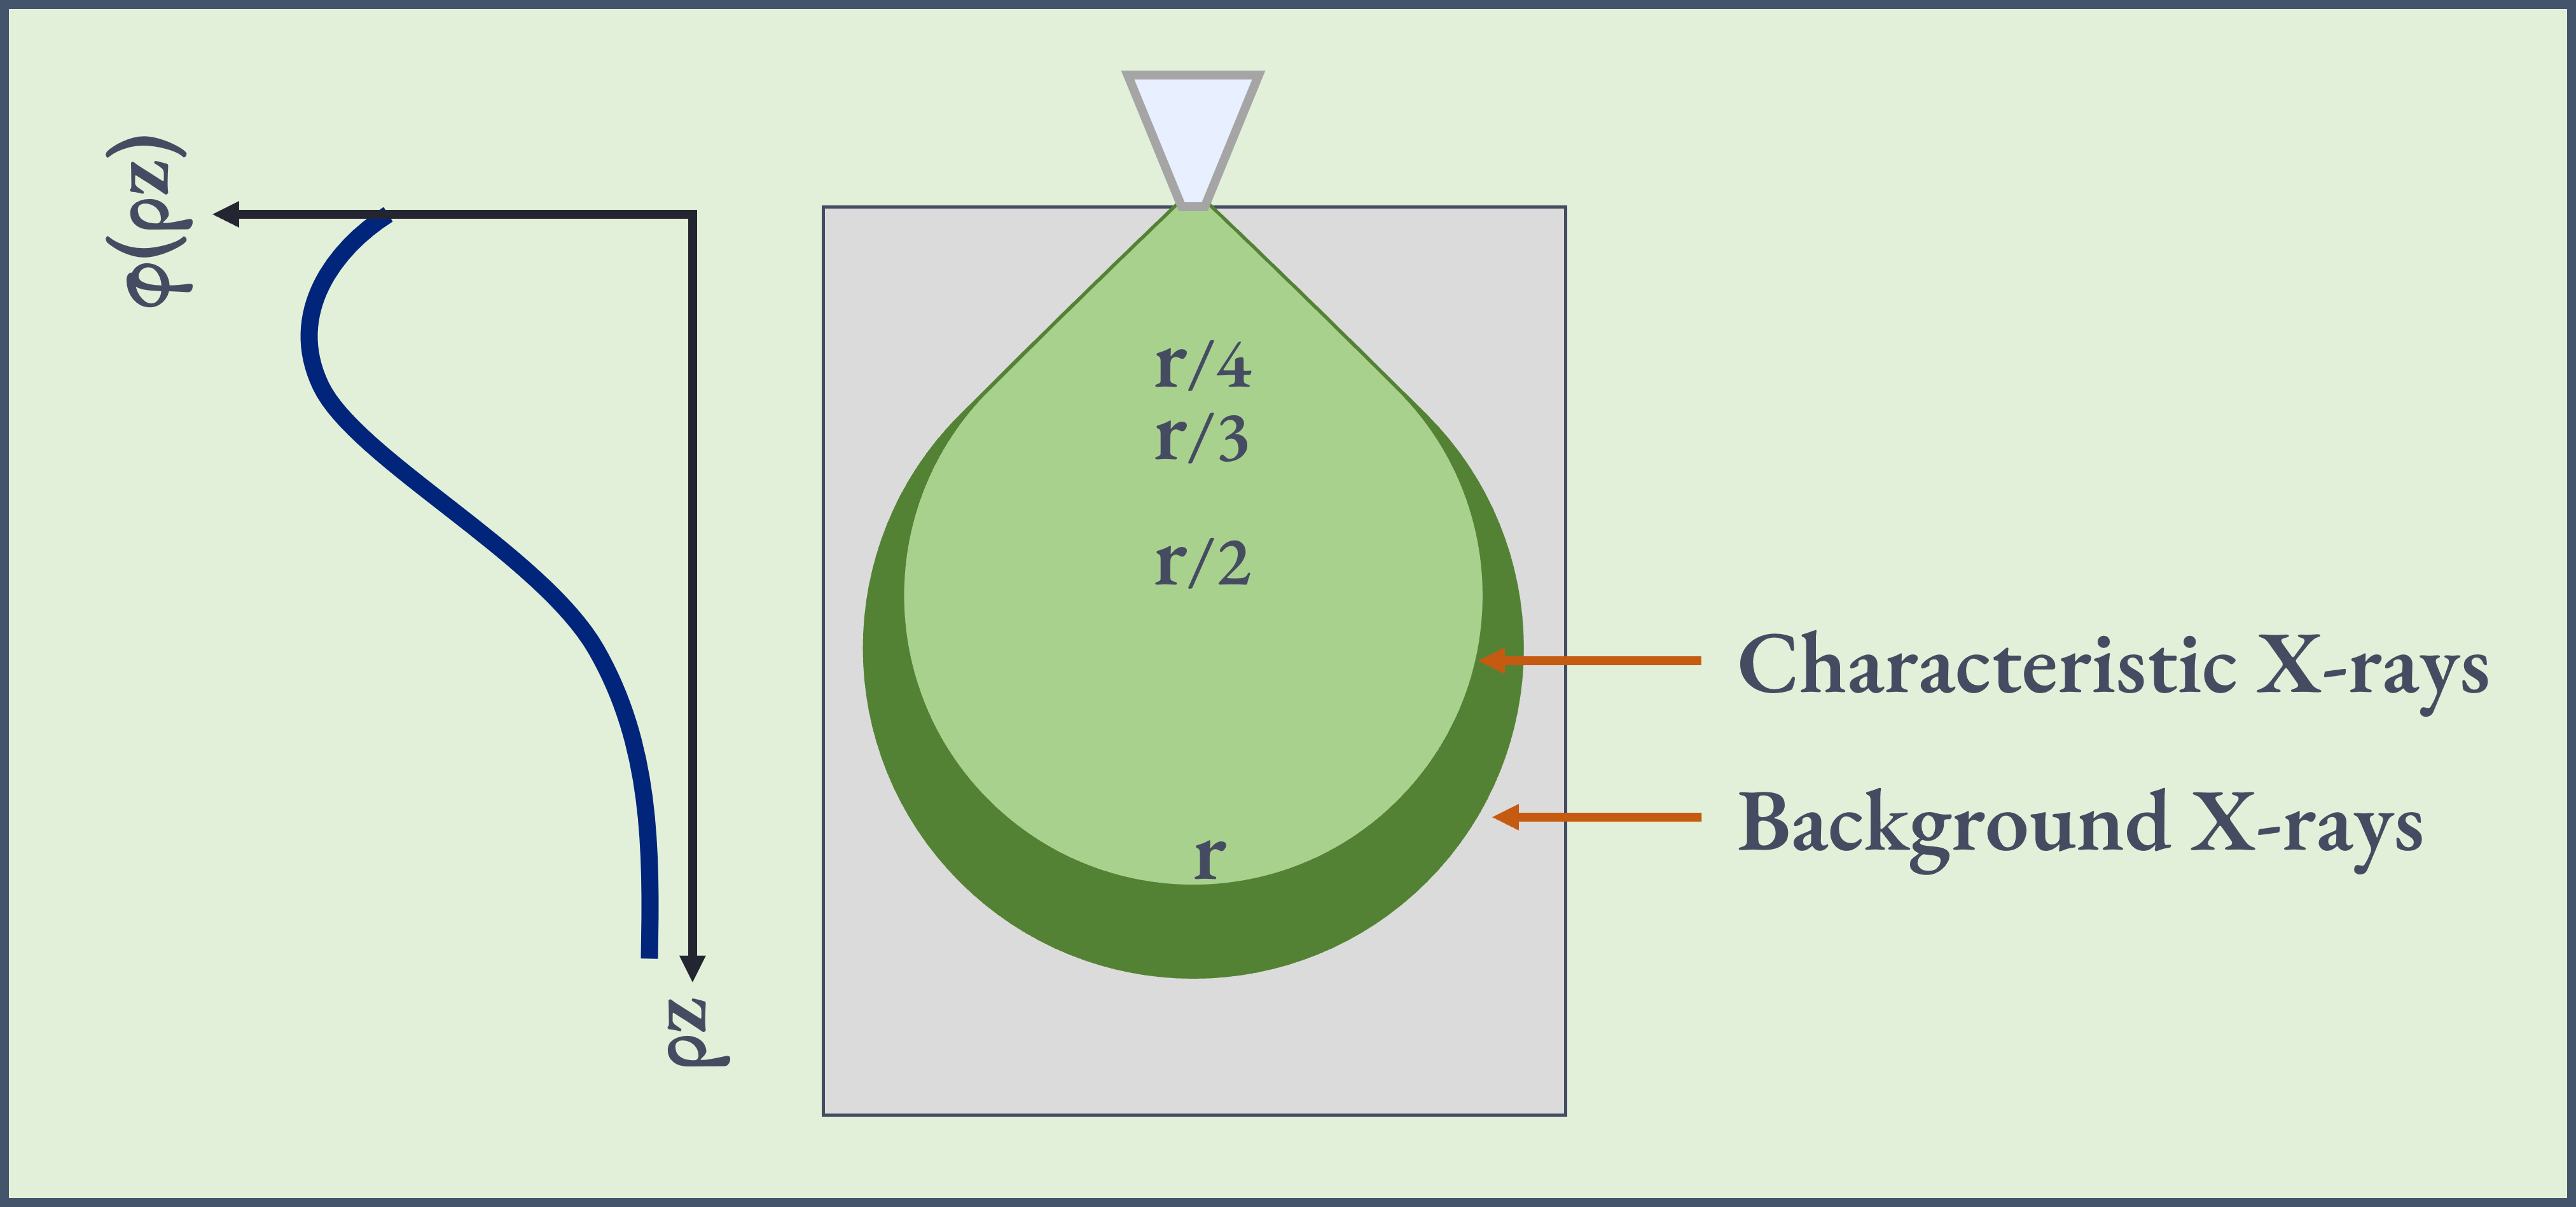
\includegraphics[width=0.8\linewidth]{figures/discussion/phi_rhoz_illustrated_with_interaction_volume.png}
    \caption{
        Illustration of the $\phi (\rho z)$ curve, with the interaction volume and the three selected average points for the ZAF absorption correction.
        The trapezoid is the incident electron beam.
        Adapted from \cite[Fig. 19.7]{goldstein_scanning_2018}.
    }
    \label{fig:discussion:depth_generation_iv}
\end{figure}

% DONE discuss: the ZAF A corrections are not good enough, at lest with the average point method tested in this work.
% DONE discuss on selected average point: maybe this approximation is severely wrong. Monte Carlo simulations show a skew towards z=0, and the numbers from HS is big. However, testing different numbers for r did not give any other more satisfactory results. Also, the phi-rho-z curves show that there is a skew towards z=0, at Rc.}
The $\phi (\rho z)$ curve is the intensity from different mass depths in the specimen, which is illustrated in \cref{fig:discussion:depth_generation_iv} and plotted with calculated data in \cref{fig:theory:quantification:phi_rho_z_curves}.
Using the parameterization of $\phi (\rho z)$ from the XPP model (\cref{eq:theory:quantitative:pap:phi_of_rho_z}), the curve for Ga L$\alpha$ is plotted in \cref{fig:discussion:pap:phi_of_rhoz}, at different beam energies.
As this figure shows, the curves are dependent on the beam energy.
The dependence on $E_0$ is explained in \cref{theory:sem:sem_signals}, and showed with numbers from the Kanaya-Okayama parameterization for electron range in \cref{tab:results:ZAF_corrections_range_r}.
The $\phi (\rho z)$ curves have a skew towards the surface where $z = \rho z = 0$.
The absorption corrections done with the ZAF model show that dividing the maximum generation depth by $2$ or $3$ did not work as well as dividing by $4$.
This is an indication that the method might provide reasonable results, if a better average point is used.
However, using a method like this with an average point might be a too simple model.


% the results
The compositional results presented in \cref{tab:results:ZAF_corrections_compositions_stats} show that the GaAs quantifications are improved by applying the ZAF absorption corrections, but the GaSb results are not.
Dividing r by a higher number made the results closer to the reference values, with an average $7$ at.\% deviation for GaAs, which is improved from $11$ at.\% deviation in the uncorrected intensity ratio results.
These results show that one of the issues with the GaAs specimen is probably absorption, and that the ZAF absorption corrections can push the results in the right direction.
However, the GaSb results increase from a $6$ at.\% deviation in the uncorrected results to a $30$ at.\% deviation with $r/2$, which decrease to a $21$ at.\% deviation with $r/4$.
This is an indication that the GaSb specimen have other issues than absorption.


% why GaAs has absorption issues
The absorption issues in the GaAs specimen can be explained by how close the As lines are to the Ga lines.
As discussed earlier, the absorption of As in GaAs is very high.
The atomic number difference between Ga and As is just $2$, thus giving the element similar physical properties for generation of X-rays.


% why GaSb has other issues
The GaSb specimen have other issues as pointed out earlier, e.g. in \cref{discussion:quantitative:initial_quantification}.
The atomic number difference of $20$ makes the generation properties more different for Ga and Sb compared to Ga and As.
This may be part of the explanation why the absorption corrections did not improve the results for GaSb.
The absorption in GaSb is high, as shown in \cref{fig:mass_absorption_coefficients}, but the results show that corrections for absorption alone is not sufficient for GaSb (see \cref{theory:quantitative:zaf}).
The best correction for GaSb might include a combination of absorption and other corrections, but the assumption given in Goldstein \cite[p. 300]{goldstein_scanning_2018} that the two effects of Z cancel each other out is not valid for GaSb.
One of the corrections applied from the XPP model is investigating the possibility for Z corrections, and the other XPP correction combines Z and A corrections.

% why GaAs still is off with the ZAF corrections.
% DONE discuss: mu_rho is taken from HS, and slight deviations can give large impacts, as mu_rho is in the exponent. ref to eq. in theory. 
Even though the ZAF absorption corrections improved the results for GaAs, the results are deviating too much from the reference values to be regarded as useful.
Possible reasons for this is the aforementioned issues with the average point, or that the input parameters for the model is not good enough.
The most important input parameter is probably the mass absorption coefficient $\mu_\rho$.
In the absorption correction (\cref{eq:theory:quantitative:absorption}), $\mu_\rho$ is used in the exponent, and small deviations in $\mu_\rho$ can give large impacts on the results.
A more detailed discussion of $\mu_\rho$ is given in \cref{discussion:quantitative:xpp}, as $\mu_\rho$ is also used in the XPP model.


% DONE discuss: my model is not reality. I had a bug for the range r, and when i fixed in the GaAs quantification was actually deviating more.
Another possible reason for the deviation is the implementation of the ZAF correction, which may have bugs in the code.
For example, the first implementation of the range $r$ was wrong, and when it was fixed, the quantification results for GaAs was actually worse.
This show that using $50:50$ as the reference to evaluate the results can be misleading, and that more testing is needed to verify the usefulness of the code developed in this work.
The code is implemented with both the purpose of testing different possibilities for corrections, and to be used as a starting point for future works.
The implementation is done to the author's best knowledge, but there is no guarantee that the code is bug free.
Additionally, every model is a simplification of reality, and the models used in this work are no exception.
The assumptions and simplifications made in the ZAF correction model in this work does seem to be on track for GaAs, but still having plenty of room for improvements.

% DONE conc: bugs are ugs. not guaranteed to be bug free.
% DONE conc: ZAF A, "This is an indication that the method might provide reasonable results, if a better average point is used. However, using a method like this with an average point might be a too simple model." Improves GaAs, but not GaSb
% DONE conc: the assumtion that the two effects of Z cancel each other out is aparently not valid for GaSb.




\subsection{XPP bulk corrections}
\label{discussion:quantitative:xpp}

Implementation of the XPP model from the PAP paper \cite{pap_1991} gave the possibility to plot the depth distribution $\phi(\rho z)$, and to calculate more advanced correction factors than the ZAF model, with multiple input parameters.
The XPP model is using fundamental physical concepts to get an accurate description of the X-ray generation and emittance in the specimen, treating correction factors in a single framework.
The corrections from the XPP model applied to the measured intensities did not give as good results as the AZtec software, which supposedly is using the same model.
This difference is probably due to implementation differences, and is discussed after the plots of the $\phi(\rho z)$ curves.

% DONE discussion: add PAP $\phi(\rho z)$ curves.
While implementing physical models, it is useful to plot the results from different steps in the model to verify that the implementation is correct.
Such plots can both be compared to figures in textbooks or papers, and can be used to reason about the results.
Code bugs are easier to reveal when parts of the code can be tested separately.
Plots of the steps in the XPP model are shown in \cref{theory:quantitative:pap}, which can be compared to the plots in the PAP paper \cite{pap_1991}.
Plotting $\phi(\rho z)$ can be done with the parameters $A$, $B$, $a$, $b$ and $\phi(0)$, using \cref{eq:theory:quantitative:pap:phi_of_rho_z}.
\cref{fig:discussion:pap:phi_of_rhoz} is a plot of $\phi(\rho z)$ for Ga L$\alpha$ in Ga, with beam energy $30$ kV, $15$ kV, $10$ kV and $5$ kV.

% figures/PAP_phi_of_rhoz.pdf
\begin{figure}[htbp]
    \centering
    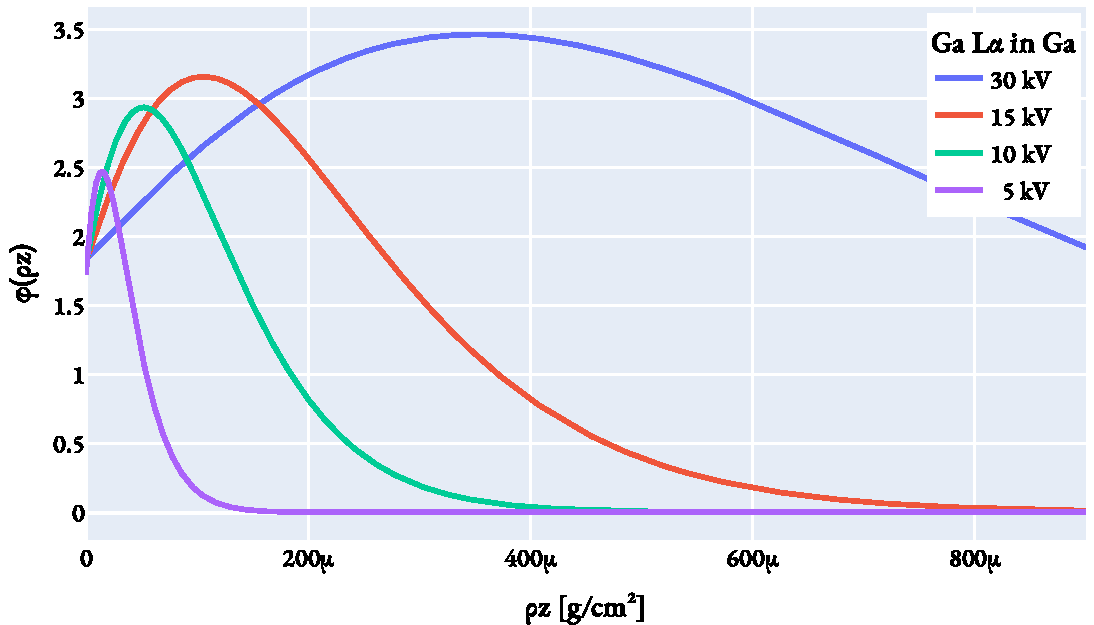
\includegraphics[width=0.8\linewidth]{figures/discussion/PAP_phi_of_rhoz.pdf}
    \caption{
        Plot of $\phi(\rho z)$ for Ga L$\alpha$ in Ga.
        The curve is calculated with \cref{eq:theory:quantitative:pap:phi_of_rho_z}.
        The plot shows three different beam energies, $30$ kV (blue), $15$ kV (red), $10$ kV (green), and $5$ kV (purple).
    }
    \label{fig:discussion:pap:phi_of_rhoz}
\end{figure}


The plot of the depth distribution $\phi(\rho z)$ in \cref{fig:discussion:pap:phi_of_rhoz} can be compared to plots in the PAP paper\cite{pap_1991}, which illustrates that the implementation of the XPP model is working mostly as intended.
Other comparisons were done, for example with figure 1 and 2 in the PAP paper, where $\phi(\rho z)$ of C K$\alpha$ in C and W are plotted.
This plot is shown in \cref{fig:discussion:pap:phi_of_rhoz_C_Ka}, where the general trend is equal to the plot in the PAP paper, but there are some differences, for example that the curve in C is rounder and broader in the PAP paper.
The plotting of $\phi(\rho z)$ was also compared to other sources, for example figure 19.9 in Goldstein \cite[Fig. 19.9]{goldstein_scanning_2018}, which is adapted in \cref{fig:theory:quantification:phi_rho_z_curves}.
The plotting of $\phi(\rho z)$ in Goldstein is done with the PROZA model, but the results should be similar to the XPP model.
\cref{fig:theory:quantification:phi_rho_z_curves} and \cref{fig:discussion:pap:phi_of_rhoz_Goldstein} are in general similar, but slight differences between $\phi(0)$ and the shape at the end of the curve can be seen, where the XPP model gives the curve a longer tail.
These plots show that the implementation of the XPP model is not perfect, but should be close enough to be useful.
Possible sources of deviation is discussed towards the end of this section.
% DONE conc: "These plots show that the implementation of the XPP model is not perfect, but should be close enough to be useful."

% figures/PAP_phi_of_rhoz_C_Ka.pdf
\begin{figure}[htbp]
    \centering
    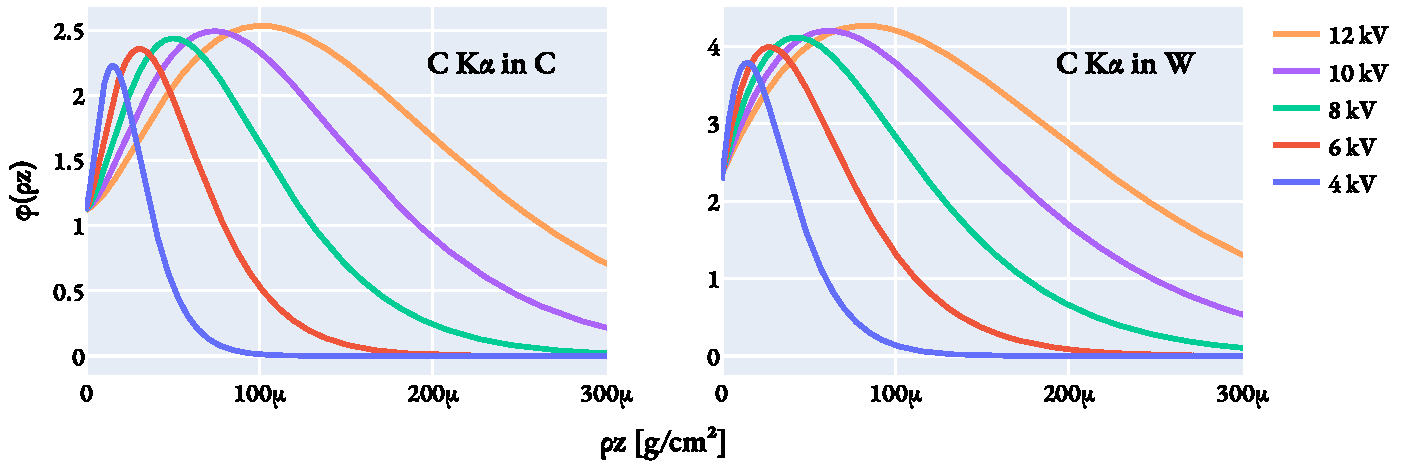
\includegraphics[width=0.99\linewidth]{figures/discussion/PAP_phi_of_rhoz_C_Ka.pdf}
    \caption{
        Plot of $\phi(\rho z)$ for C K$\alpha$ in C and W, at different beam energies.
        The plot is used to compare the implementation of the XPP model to the PAP paper \cite[Fig. 1 and 2]{pap_1991}.
    }
    \label{fig:discussion:pap:phi_of_rhoz_C_Ka}
\end{figure}



% figures/PAP_phi_of_rhoz_Goldstein.pdf
\begin{figure}[htbp]
    \centering
    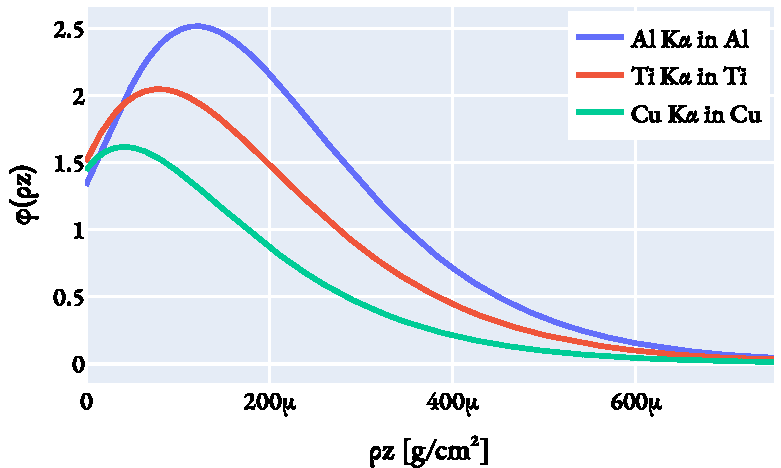
\includegraphics[width=0.7\linewidth]{figures/discussion/PAP_phi_of_rhoz_Goldstein.pdf}
    \caption{
        Plot of $\phi(\rho z)$ from the XPP model for Al K$\alpha$ in Al, Ti K$\alpha$ in Ti, and Cu K$\alpha$ in Cu, with beam energy $15$ kV.
        Comparison of the plot can be done with \cref{fig:theory:quantification:phi_rho_z_curves}, which is an adapted figure from Goldstein \cite[Fig. 19.9]{goldstein_scanning_2018}.
    }
    \label{fig:discussion:pap:phi_of_rhoz_Goldstein}
\end{figure}




% The correctios done with XPP
Two type of bulk corrections from the XPP model were implemented and tested, one which only corrected for the calculated generation of X-rays, and one which corrected for the ratio between the emitted and generated signal, i.e. the absorption factor.
The first correction divide the measured intensity by $F$ (see \cref{theory:quantitative:pap:calculation_of_F}), which the area of the $\phi(\rho z)$ curve, i.e. the generated signal.
This correction is supposed to correct for different Z, and should cover differences in factors like the critical ionization energy (see \cref{theory:xray_formation:energy}), and fluorescence yield (see \cref{fig:theory:fluorescence_yield}). 
The second correction divide the measured intensity by $f(\chi)$ (see \cref{eq:theory:quantitative:pap:absorption_correction}), which is the XPP absorption factor.
The correction with $f(\chi)$ is supposed to correct for both Z and A, as the calculated absorption factor is dependent on both $F$ and $F(\chi)$, where $F(\chi)$ is the $\phi(\rho z)$ curve with absorption correction in each layer.
$F$ and $F(\chi)$ are illustrated in \cref{fig:discussion:pap:F_and_Fchi}.
The two corrections were tested because of the implications of the previously discussed results, where GaAs probably need absorption corrections, while GaSb also need corrections for different Z.

% figures/discussion/xpp_absorption_correction.png
\begin{figure}[hbtp]
    \centering
    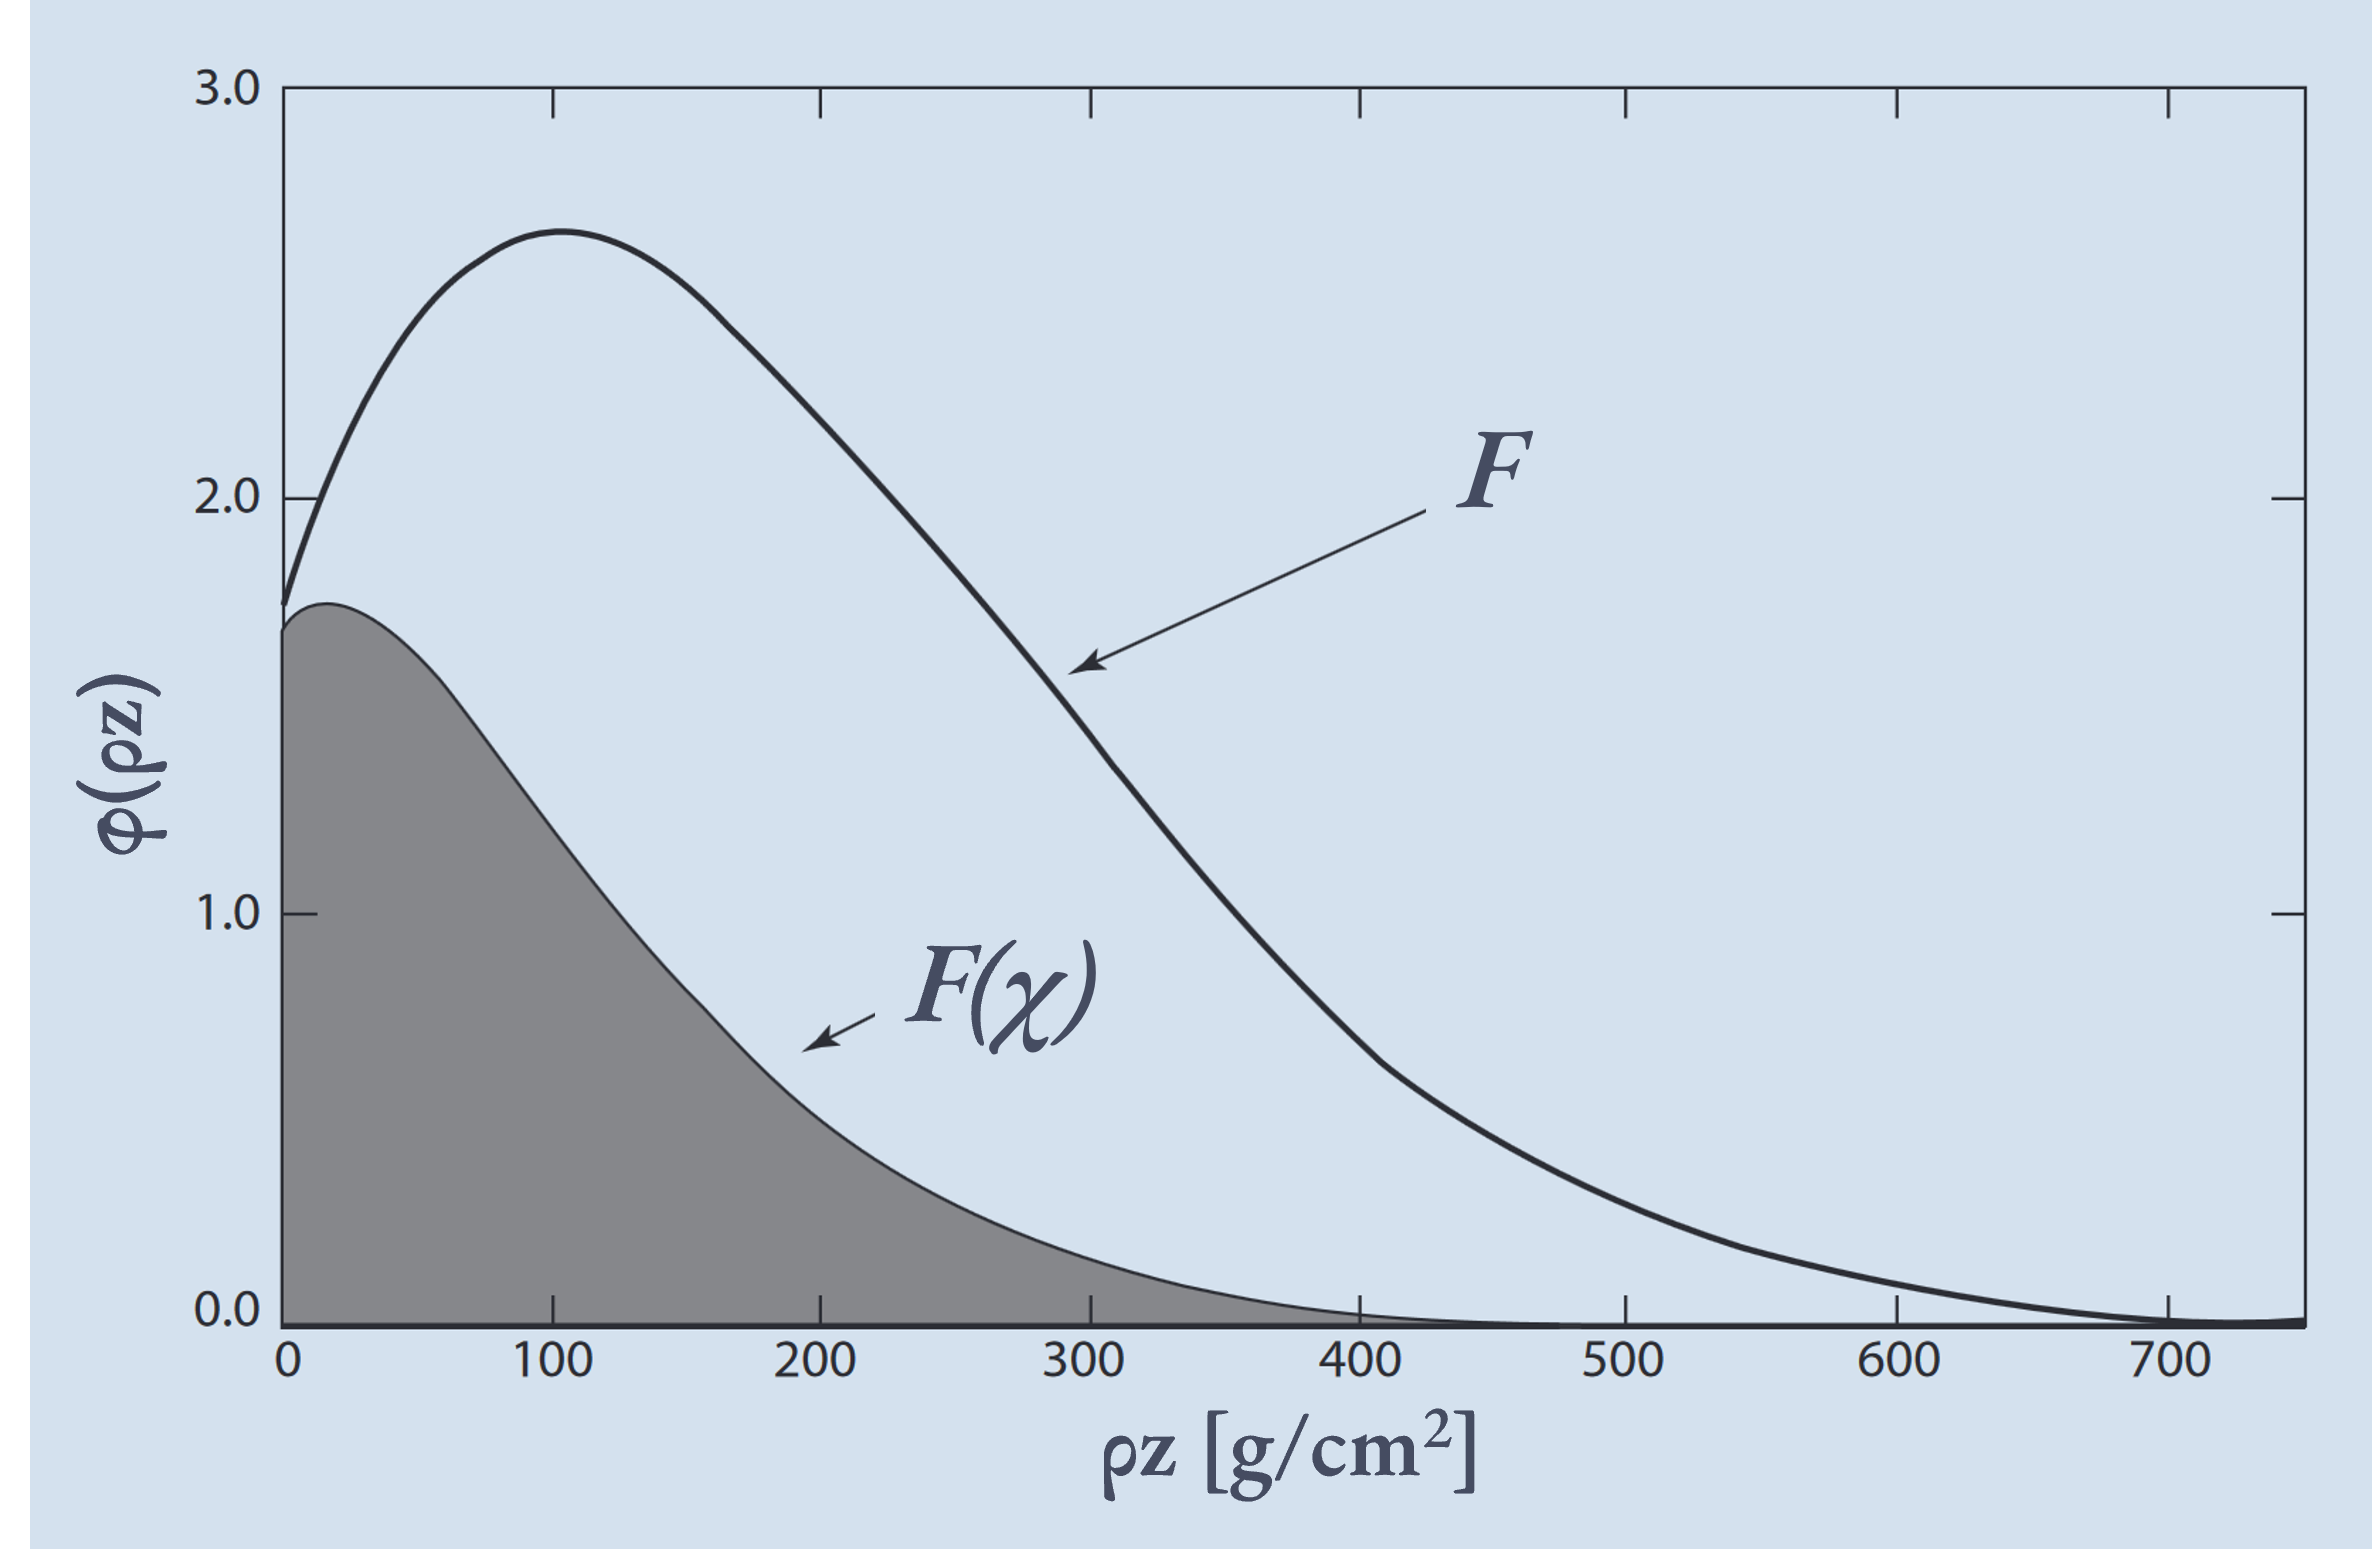
\includegraphics[width=0.75\linewidth]{figures/discussion/xpp_absorption_correction.png}
    \caption{
        Illustration of $F$ and $F(\chi)$.
        $F$ is the area of the $\phi(\rho z)$ curve, while $F(\chi)$ is the area of the $\phi(\rho z)$ curve with absorption correction in each layer.
        $F$ is the generated signal, while $F(\chi)$ is the emitted signal.
        $f(\chi) = F(\chi) / F$ is the absorption factor.
        The $\phi(\rho z)$ curve is for Al K$\alpha$ in a Cu matrix at $E_0 = 20$ keV.
        Adapted from \cite[Fig. 19.14]{goldstein_scanning_2018}.
    }
    \label{fig:discussion:pap:F_and_Fchi}
\end{figure}


% the results
The corrections with the XPP model presented in \cref{tab:results:XPP_compositions_stats} show that the corrections needed differ between the two specimen.
This was expected, as the materials have different properties for generation and absorption of X-rays.
% GaAs
The GaAs specimen is corrected best with $f(\chi)$, and the results from this absorption correction is better than from the ZAF correction.
The $F$ correction on GaAs from the uncorrected results is only giving an improvement from $12$ at.\% to $11$ at.\%.
This is an implication that the Z effects alone are not that strong in GaAs, but when the Z effect is added to the absorption effect, the results are improved.
% GaSb
The GaSb specimen is corrected best with $F$, which implies that the Z effects are most important for this specimen.
As the results show, the $10$ kV and $15$ kV GaSb spectrum are corrected quite nicely with the $F$ correction, but the $30$ kV spectrum is pushed away from the reference value.
Overall, the average quantification deviation in GaSb is both $6$ at.\% at the uncorrected and the $F$ corrected results, while the $f(\chi)$ corrected results have a large deviation at $38$ at.\%.

% DONE conc: Two corrections tested from the XPP model, one for only Z and one for Z and A (whole). GaAs is best corrected with f(chi), while GaSb is best corrected with F.

% why the large deviation in GaSb? mu_rho
% Possible source of error for my implementation of the PAP model:
The large deviation in the $f(\chi)$ corrected results for GaSb is probably caused by the $\mu_\rho$ values used in the calculation of $F(\chi)$.
Section II.E in the PAP paper is discussing the absorption coefficients for the PAP model, and Appendix 5 \cite[p. 63]{pap_1991} in the paper lists some values for $\mu_\rho$ associated with the PAP procedure.
These numbers are in the same range as the numbers provided by HyperSpy, but there are deviations.
All the following examples for $\mu_\rho$ are in units of cm$^2$/g.
For example, the line As L$\alpha$ in GaAs bulk is given $\mu_\rho = 7000$ in the PAP paper, and the value $\mu_\rho = 3744$ by HyperSpy.
Cu L$\alpha$ in pure Cu is given $\mu_\rho = 1755$ in the PAP paper, and $\mu_\rho = 1515$ by HyperSpy.
Cu L$\beta$ in pure Cu is given $\mu_\rho = 6750$ in the PAP paper, while HyperSpy give $\mu_\rho = 8763$ for Cu L$\beta_1$.
These deviations are almost certainly a source of error, which should lead to some adjustments of the XPP equations.
As explained in \cref{discussion:quantitative:zaf_absorption_correction}, the value of $\mu_\rho$ is critical because it is in the exponent of the absorption calculation.
Such corrections might have been published as an update to the PAP/XPP procedure in a more recent paper.
If this is a source of error, it can explain why the AZtec software is getting better results, because Oxford Instruments have had time to refine their input parameters and equations.
In this work, the $\mu_\rho$ values from HyperSpy were used, and as the package is emergent from the TEM community, the values could be less accurate at low voltages.
The original source is NIST standard reference database 66, mentioned in \cref{theory:xray_formation:characteristic}, where it is stated in the documentation of the database that the values are less accurate between $0.03$ keV to $3$ keV, and around absorption edges \cite{nist_xraydatabase_hyperspy}.
Further, the documentation to the NIST database state that revised values for $\mu_\rho$ can lead to "significant qualitative and quantitative improvement" \cite{nist_xraydatabase_hyperspy}\footnote{\url{https://www.nist.gov/pml/nist-x-ray-form-factor-attenuation-and-scattering-tables-database-cont}, accessed 26.05.23.}.
Investigating such possibilities are outside scope of this work, but can be a starting point for future work.


% using different corrections tailored for different specimen
The results from the two specimen show that the corrections needed are not universal.
Correcting for absorption when it is not needed can lead to worse results, as seen in the GaSb specimen.
The best results for the GaAs spectra is obtained with a combination of Z and A effects through the $f(\chi)$ correction, while the best results for the GaSb spectra is obtained with the Z effect through the $F$ correction.
This implies that the best results are obtained by using different corrections tailored for different specimen.
It may be that such a solution is implemented in the AZtec software, for example that absorption effects are taken into account if certain conditions are met.
Even though Oxford Instruments refer to the XPP model in the original PAP paper, they have definitely made continuous improvements and adjustments to their commercial software.
Refining input parameters and adjusting the equations requires extensive testing and validation on different elements and specimen.
Just testing different elements is not enough, as seen in the results where the Ga signal is behaving differently depending on the other element in the specimen.
With the right corrections applied to the specimen of interest, the quantitative EDS results can be improved.
Such corrections should be in an open-source software package, where the documentation is clear, and the code is available for inspection and modification.
This would allow better EDS results and more reliable quantification, leading to higher quality research from the EDS community.


% DONE: analytical vs numerical solutions. 
Another possible improvement to the XPP model is to use numerical solutions instead of analytical solutions.
The original PAP paper is using analytical solutions to the equations, but with the computer power available in standard computers today, the equations could be solved numerically.
This could lead to more accurate results, as the analytical solutions are approximations of the numerical solutions.
Testing out numerical calculations of the $\phi(\rho z)$ curves can be done in future works, to see if the corrections can be improved.

% DONE discuss: Other methods, such as the PROZA96 model, could be tested in future works, using the code developed in this work as a starting point, because there are overlapping parts between the models.
Yet another possibility is to test other correction models, such as the PROZA96 model \cite{bastin_proza96_1998}.
Testing the PROZA96 model can be done with the code developed in this work as a starting point, because there are overlapping parts between the models.
The paper by Bastin et al. \cite{bastin_proza96_1998} which presents the PROZA96 model is referring to the PAP paper for calculations of the area $F$ of the $\phi(\rho z)$ curves.
This code can be copied from the XPP model.
However, if the main issue is the input parameters like the $\mu_\rho$ values, the PROZA96 model might suffer from the same problems as the XPP model developed in this work.
Other models which are not based on relative intensities, like the PAP and PROZA96 models, could also be tested in future works.
% TODO discuss: the F and f(chi) is calculated for relative intensities. To calculate absolute number of X-rays generated, the probe current must be know. That was not possible in this project. Calculations of absoule generated X-rays are done in e.g. the Zeta method for thin films.
Such models, like the Zeta method for thin specimen \cite[Ch. 35.5]{williams_carter_tem_2009}, require the probe current as an input parameter.
Measuring the probe current is not possible with the equipment available in this work, but a Faraday cup could be installed in the SEM to test out such models \cite{goldstein_scanning_2018}.












\subsection{Bulk correction summary}
\label{discussion:quantitative:summary}


SEM EDS analysis through AZtec can provide accurate results, which are better than the bulk corrected results from the XPP model implemented in this work.
The XPP model implemented in this work is far from finished, but it is a starting point for future work.
Earlier attempts\footnote{Issue \#800: \url{https://github.com/hyperspy/hyperspy/issues/800}}\footnote{Issue \#2332: \url{https://github.com/hyperspy/hyperspy/issues/2332}} have been made to implement ZAF corrections for SEM EDS quantification in HyperSpy, but these have stagnated.
The stagnation is probably in part due to the aforementioned issues with the input parameters, and that ZAF corrections may be less suited for a wide range of specimen, which $\phi (\rho z)$ corrections like the XPP model are.
In other words, bulk corrections from the XPP model are probably better suited than ZAF for HyperSpy or similar software packages.


As discussed, the model coded in this project cna be improved by refinement of the input parameters, by testing on different specimen, applying restrictions for which corrections to use in which cases, and by refining the code.
There might still be errors in the implementation, and even the interpretation of the equations to use, but the general trend of the model is an improvement of the results.
The corrections used suggest that the model is working, but still needs refinement.
The refinement needed are probably both in the input parameters and in the implementation of the equations in the notebook.
Regardless of this, the code developed and the work done is a step towards better EDS through open science.






% DONE conc: the input parameters are probably off, especially mu_rho, which is important. The numbers avaliable through hyperspy are less accurate at the relevant energies and around absorption edges, which is a critical source of error.
% TODO FW: finding better mu_rho, as they most likely have done in AZtec, would probably improve the results. This is outside the scope of this work, but can be a starting point for future work. other imput parameters could also need refinement, but mu_rho is really important and does for sure need refinement.

% DONE conc: a complete correction program must give different corrections to different specimen. If absorption is an issue, eg. with similar Z, is must be corrected. And if Z distance is large, the Z effects play a role. AZtec is most likely doing such selections, but that is unknown.

% TODO FW: refine the XPP model. It works in AZtec pretty well, so it should work, but might need to compensate differently with different compositions.

% TODO FW: do the XPP calculations analytically, might improve the results. Should be possible with standard modern computers.

% TODO FW: test other correction models, like PROZA96. The code here can be a start, as F is reused from the PAP model. Also test absolute models, where the probe current is measured with a Faraday cup.

% DONE conc: main XPP, the work done here is a start, but not a finished model. Refining parameters and equations, squashing bugs, and extensive testing is needed. The general trend is that the model is correct, but not perfect. Even so, this work is a step towards better EDS through open science.

